\documentclass{article}

% packages
  % basic stuff for rendering math
  \usepackage[letterpaper, top=1in, bottom=1in, left=1in, right=1in]{geometry}
  \usepackage[utf8]{inputenc}
  \usepackage[english]{babel}
  \usepackage{amsmath} 
  \usepackage{amssymb}
  % \usepackage{amsthm}

  % extra math symbols and utilities
  \usepackage{mathtools}        % for extra stuff like \coloneqq
  \usepackage{mathrsfs}         % for extra stuff like \mathsrc{}
  \usepackage{centernot}        % for the centernot arrow 
  \usepackage{bm}               % for better boldsymbol/mathbf 
  \usepackage{enumitem}         % better control over enumerate, enumerate
  \usepackage{hyperref}         % for hypertext linking
  \usepackage{fancyvrb}          % for better verbatim environments
  \usepackage{newverbs}         % for texttt{}
  \usepackage{xcolor}           % for colored text 
  \usepackage{listings}         % to include code
  \usepackage{lstautogobble}    % helper package for code
  \usepackage{parcolumns}       % for side by side columns for two column code
  \usepackage{xfrac}
  \usepackage{bbm, dsfont}
  % page layout
  \usepackage{fancyhdr}         % for headers and footers 
  \usepackage{lastpage}         % to include last page number in footer 
  \usepackage{parskip}          % for no indentation and space between paragraphs    
  \usepackage[T1]{fontenc}      % to include \textbackslash
  \usepackage{footnote}
  \usepackage{etoolbox}
  \usepackage{anyfontsize}

  % for custom environments
  \usepackage{tcolorbox}        % for better colored boxes in custom environments
  \tcbuselibrary{breakable}     % to allow tcolorboxes to break across pages

  % figures
  \usepackage{pgfplots}
  \pgfplotsset{compat=1.18}
  \usepackage{float}            % for [H] figure placement
  \usepackage{tikz}
  \usepackage{tikz-cd}
  \usepackage{circuitikz}
  \usetikzlibrary{arrows}
  \usetikzlibrary{positioning}
  \usetikzlibrary{calc}
  \usepackage{graphicx}
  \usepackage{caption} 
  \usepackage{subcaption}
  \captionsetup{font=small}
  \usepackage{booktabs} % For formal tables

  % for tabular stuff 
  \usepackage{dcolumn}

  \usepackage[nottoc]{tocbibind}
  \pdfsuppresswarningpagegroup=1
  \hfuzz=5.002pt                % ignore overfull hbox badness warnings below this limit

% New and replaced operators
  \DeclareMathOperator{\Tr}{Tr}
  \DeclareMathOperator{\Sym}{Sym}
  \DeclareMathOperator{\Span}{span}
  \DeclareMathOperator{\std}{std}
  \DeclareMathOperator{\Cov}{Cov}
  \DeclareMathOperator{\Var}{Var}
  \DeclareMathOperator{\Corr}{Corr}
  \DeclareMathOperator{\pos}{pos}
  \DeclareMathOperator{\MV}{MV}
  \DeclareMathOperator{\V}{V}
  \DeclareMathOperator*{\argmin}{\arg\!\min}
  \DeclareMathOperator*{\argmax}{\arg\!\max}
  \newcommand{\ket}[1]{\ensuremath{\left|#1\right\rangle}}
  \newcommand{\bra}[1]{\ensuremath{\left\langle#1\right|}}
  \newcommand{\braket}[2]{\langle #1 | #2 \rangle}
  \newcommand{\qed}{\hfill$\blacksquare$}     % I like QED squares to be black

% Custom Environments
  \newtcolorbox[auto counter, number within=section]{question}[1][]
  {
    colframe = orange!25,
    colback  = orange!10,
    coltitle = orange!20!black,  
    breakable, 
    title = \textbf{Question \thetcbcounter ~(#1)}
  }

  \newtcolorbox[auto counter, number within=section]{exercise}[1][]
  {
    colframe = teal!25,
    colback  = teal!10,
    coltitle = teal!20!black,  
    breakable, 
    title = \textbf{Exercise \thetcbcounter ~(#1)}
  }
  \newtcolorbox[auto counter, number within=section]{solution}[1][]
  {
    colframe = violet!25,
    colback  = violet!10,
    coltitle = violet!20!black,  
    breakable, 
    title = \textbf{Solution \thetcbcounter}
  }
  \newtcolorbox[auto counter, number within=section]{lemma}[1][]
  {
    colframe = red!25,
    colback  = red!10,
    coltitle = red!20!black,  
    breakable, 
    title = \textbf{Lemma \thetcbcounter ~(#1)}
  }
  \newtcolorbox[auto counter, number within=section]{theorem}[1][]
  {
    colframe = red!25,
    colback  = red!10,
    coltitle = red!20!black,  
    breakable, 
    title = \textbf{Theorem \thetcbcounter ~(#1)}
  } 
  \newtcolorbox[auto counter, number within=section]{proposition}[1][]
  {
    colframe = red!25,
    colback  = red!10,
    coltitle = red!20!black,  
    breakable, 
    title = \textbf{Proposition \thetcbcounter ~(#1)}
  } 
  \newtcolorbox[auto counter, number within=section]{corollary}[1][]
  {
    colframe = red!25,
    colback  = red!10,
    coltitle = red!20!black,  
    breakable, 
    title = \textbf{Corollary \thetcbcounter ~(#1)}
  } 
  \newtcolorbox[auto counter, number within=section]{proof}[1][]
  {
    colframe = orange!25,
    colback  = orange!10,
    coltitle = orange!20!black,  
    breakable, 
    title = \textbf{Proof. }
  } 
  \newtcolorbox[auto counter, number within=section]{definition}[1][]
  {
    colframe = yellow!25,
    colback  = yellow!10,
    coltitle = yellow!20!black,  
    breakable, 
    title = \textbf{Definition \thetcbcounter ~(#1)}
  } 
  \newtcolorbox[auto counter, number within=section]{example}[1][]
  {
    colframe = blue!25,
    colback  = blue!10,
    coltitle = blue!20!black,  
    breakable, 
    title = \textbf{Example \thetcbcounter ~(#1)}
  } 
  \newtcolorbox[auto counter, number within=section]{code}[1][]
  {
    colframe = green!25,
    colback  = green!10,
    coltitle = green!20!black,  
    breakable, 
    title = \textbf{Code \thetcbcounter ~(#1)}
  } 

  \BeforeBeginEnvironment{example}{\savenotes}
  \AfterEndEnvironment{example}{\spewnotes}
  \BeforeBeginEnvironment{lemma}{\savenotes}
  \AfterEndEnvironment{lemma}{\spewnotes}
  \BeforeBeginEnvironment{theorem}{\savenotes}
  \AfterEndEnvironment{theorem}{\spewnotes}
  \BeforeBeginEnvironment{corollary}{\savenotes}
  \AfterEndEnvironment{corollary}{\spewnotes}
  \BeforeBeginEnvironment{proposition}{\savenotes}
  \AfterEndEnvironment{proposition}{\spewnotes}
  \BeforeBeginEnvironment{definition}{\savenotes}
  \AfterEndEnvironment{definition}{\spewnotes}
  \BeforeBeginEnvironment{exercise}{\savenotes}
  \AfterEndEnvironment{exercise}{\spewnotes}
  \BeforeBeginEnvironment{proof}{\savenotes}
  \AfterEndEnvironment{proof}{\spewnotes}
  \BeforeBeginEnvironment{solution}{\savenotes}
  \AfterEndEnvironment{solution}{\spewnotes}
  \BeforeBeginEnvironment{question}{\savenotes}
  \AfterEndEnvironment{question}{\spewnotes}
  \BeforeBeginEnvironment{code}{\savenotes}
  \AfterEndEnvironment{code}{\spewnotes}

  \definecolor{dkgreen}{rgb}{0,0.6,0}
  \definecolor{gray}{rgb}{0.5,0.5,0.5}
  \definecolor{mauve}{rgb}{0.58,0,0.82}
  \definecolor{lightgray}{gray}{0.93}

  % default options for listings (for code)
  \lstset{
    autogobble,
    frame=ltbr,
    language=C,                           % the language of the code
    aboveskip=3mm,
    belowskip=3mm,
    showstringspaces=false,
    columns=fullflexible,
    keepspaces=true,
    basicstyle={\small\ttfamily},
    numbers=left,
    firstnumber=1,                        % start line number at 1
    numberstyle=\tiny\color{gray},
    keywordstyle=\color{blue},
    commentstyle=\color{dkgreen},
    stringstyle=\color{mauve},
    backgroundcolor=\color{lightgray}, 
    breaklines=true,                      % break lines
    breakatwhitespace=true,
    tabsize=3, 
    xleftmargin=2em, 
    framexleftmargin=1.5em, 
    stepnumber=1
  }

% Page style
  \pagestyle{fancy}
  \fancyhead[L]{Quantitative Finance}
  \fancyhead[C]{Muchang Bahng}
  \fancyhead[R]{Spring 2024} 
  \fancyfoot[C]{\thepage / \pageref{LastPage}}
  \renewcommand{\footrulewidth}{0.4pt}          % the footer line should be 0.4pt wide
  \renewcommand{\thispagestyle}[1]{}  % needed to include headers in title page

\begin{document}

\title{Quantitative Finance}
\author{Muchang Bahng}
\date{Spring 2024}

\maketitle
\tableofcontents
\pagebreak

\section{Markets}

  If we have two parties that want to exchange goods, they can meet up, decide on a price, and exchange the good. However, when it comes to many players, we must make some sort of exchange. We go over the construction of one. 

  \subsection{Counterparties and Clearing Houses}

    Think about when one party buys stocks or bonds. Their downside is limited to the amount they paid on the stock, but there are many other cases where they may not be protected. 

    \begin{definition}[Default]
      If a borrower fails to pay back a debt or cover a loss, then they \textbf{default}. 
    \end{definition}

    \begin{example}[Risks Associated with Trades]
      \begin{enumerate}
        \item The simplest case is when they are in debt. They want to borrow $X$ for a certain time, and repay it back in a year at some interest rate $X (1 + r)$. However, they may not have the money by then. 
        \item When they short a stock, they can borrow money from another party that owns the stock, sell it, and buy it back at a lower price. However, if the price of the stock rises, then they must pay even more money to buy it back, and they may not have enough money to. 
        \item When they buy a stock on margin, they borrow money from a broker to buy the stock, and they must pay back the broker with interest. However, the price of the stock may fall and the borrower, even after liquidating the stock, may not have enough money to pay back the broker.
        \item Someone who longs a forward contract may not have enough money to pay the difference between the forward price and the spot price.
      \end{enumerate}
    \end{example}

    \begin{definition}[Counterparty]
      A \textbf{counterparty} is the other party in a financial transaction. 
    \end{definition}

    Note that in a vanilla exchange, the two parties trading are counterparties to each other. This is called a \textbf{bilaterial exchange}. As we have seen, this is risky since if one party defaults, the other party is left with nothing. Therefore, the markets introduce a middleman that takes care of this risk. 

    \begin{definition}[Clearing House]
      The \textbf{clearing house} is an entity that is counterparty to all parties. This means that if party A and party B want to trade, they must go through the clearing house. The clearing house buys from B and sells to A. Therefore, the counterparty risk is now within the clearing house.
    \end{definition}

    It seems that we have simply moved the risk from the traders to the clearinghouse, and this is correct. The traders are glad that the risk is gone from them since they will always be paid by the clearinghouse, and the clearinghouse can add additional regulations on trading to reduce the risk of default. The first regulation they should impose are margin requirements. 

    \begin{definition}[Margin]
      \textbf{Margin} is simply cash or some other asset (stocks, bonds, etc.) that can be used as collateral during a trade. Note that this does not mean that the collateral must be invested into anything. It is just restricted to sit there in your bank account. 
      \begin{enumerate}
        \item Cash is the most liquid form of margin, and is the most common form of margin. 
        \item Bonds are also a common form of margin, and Treasury bonds are usually valued at 90\% of their market value.
        \item Stocks are also a common form of margin, and are usually valued at 50\% of their market value. 
      \end{enumerate}
    \end{definition}

    The margin requirements are generally very inflexible unless you have a good relationship with your broker and are a big trader. Now that we've seen the important roles that a clearing house plays, we look at the development of more complex markets, namely, the exchange and OTC markets. 

  \subsection{Exchange vs OTC Markets}

    In a trading floor or pit, there are groups of traders huddled at certain physical locations that trade a certain asset, like corn futures. Back then, there would be individual traders that have their own small capital that they can trade with, called \textbf{locals}, but they have been dominated by traders that work for large financial institutions, causing locals to be either pushed our or joined with the firms. Market making firms like Akuna have pit traders, who have headsets and tablets, that are in real-time communication with the screen traders upstairs. 

    Standing in the perimeter of the trader circle are the \textbf{brokers}, who relay orders between the traders in the pit and outside of the pit. These brokers also have devices that allow them to communicate with \textbf{off floor} parties, who are individuals that are interested in these products. 

    \begin{example}[Off Floor Parties]
      Some examples of off floor parties are: 
      \begin{enumerate}
        \item Hedge funds, who have devised trading strategies that they want to implement, e.g. using drones to look at the harvest quantity. Now they want to gain exposure to the corn market. 
        \item Banks might also want to use client money to develop a trading strategy. 
        \item Consumers such as Kellogs (which needs a lot of corn to make cereal) might be interested in buying contracts to hedge their underlying exposure. 
        \item Producers like corn farmers might want to buy some contract to lock in the price in which they can sell it at. 
        \item Large funds like pension funds or family money. 
        \item Retail investors like small, non-professional traders that might dabble in options.  
        \item Other market makers might be connected to these brokers
      \end{enumerate}
    \end{example}

    There is specific terminology that we should introduce first. 

    \begin{definition}[Bid, Offer]
      
    \end{definition}
    Now if some off floor party decides to sell some calls, they will call their broker and ask to quote some prices. This means that they are asking for bid and offer prices. These traders might quote the following prices: 



    When more people want to buy and sell things, they must go to an \textbf{exchange}, which is literally a physical space that is leased to various parties (e.g. large banks, hedge funds) so that they can exchange goods. These exchanges also collect money through fees from companies to be listed on NYSE. There are two big exchanges, the NYSE and the NASDAQ, in the U.S., both located in New York. 

    Us retail traders are not direct participants of the exchange; the parties that participate there are called the \textbf{market makers}, or \textbf{liquidity providers}. Market makers, usually large banks or financial institutions (like hedge funds), make sure that there is enough trading volume to ensure liquidity in the market. A buyer and a seller must meet together to complete a deal, and to ensure that this happens smoothly (i.e. provides liquidity), a market maker buys stocks (through the individual's brokerage) and sells them to the corresponding recipient. Essentially, they provide a pool of shares and act as intermediaries between them. They profit from the bid-ask spread, though sudden volatility is always a risk. For example, if a crash happens (i.e. a market maker buys a stock and it tanks before they can sell it), then the market makers get screwed because they are left with an undervalued stock. 

    The trader cannot directly trade through the market makers. They must contact their \textbf{broker}, which is another company that acts as an intermediary. If I want to buy a stock, my buy order gets sent to my broker, which gets sent to the market makers, which pairs me up with a seller through their own broker, and the transaction is completed. These brokers make money through commissions from the traders and from trading in dark pools, which we'll talk about later. They also give access to traders the forecasts of analyst reports for companies and other research. 

    \begin{center}
        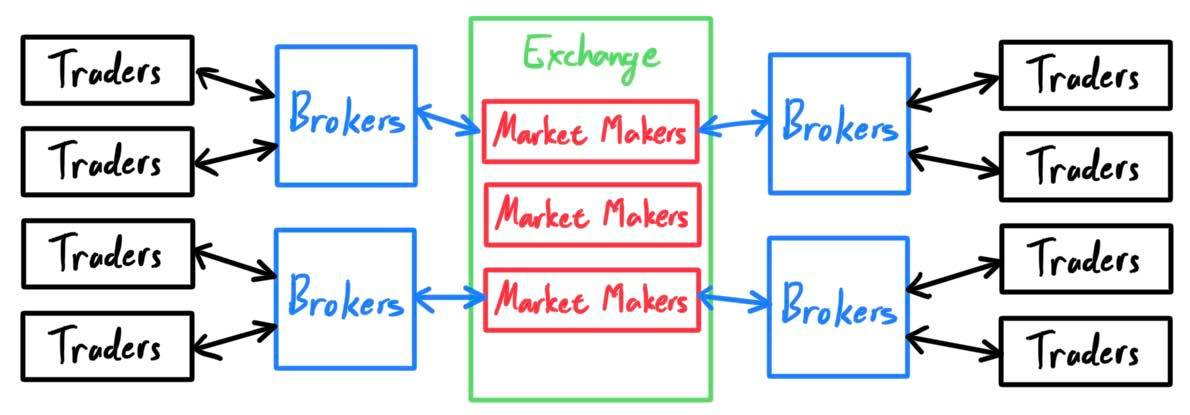
\includegraphics[scale=0.3]{img/exchange.jpg}
    \end{center}

    Clearly, there can be some shady stuff going on here, but luckily, the SEC and the FINRA consistently regulate the markets to ensure fairness for the little players (retail investors). One of the most important regulations is the 2005 Regulation NMS (National Market System), which required exchanges to publish the best bid and offer price for each stock, required them to route orders to the trading venue with the best price, and had set the minimal price quotation increment to \$0.01. This ensured transparency and protection of the investor with the best price execution (but this can be taken advantage of by high frequency traders). 

    \begin{definition}[Exchange Markets]
      \textbf{Exchange markets} are markets that exchange \textit{standardized} contracts and is \textit{highly regulated} (to protect investors) by a central authority. A buyer and seller come together to trade a contract, and they enter the contract through a \textbf{clearing house}, which is the \textit{counterparty} to all trades. That is, both the buyer and seller enter into a contract with the clearing house. Doing this reduces the counterparty risk by ensuring that both sides have adequate \textit{margin}. For example, if the buyer wins the bet and the seller can't pay, the clearing house will pay the buyer.
    \end{definition}

    \begin{question}
      Talk about counterparties, clearinghouses. 
    \end{question}

    \subsubsection{Market Making and High Frequency Trading}

      A significant mover of markets are \textbf{high frequency traders}, or HFTs. HFT is a type of algorithmic trading that are characterized by high speeds and high turnover rates. It is the primary type of algorithmic trading and consists of about 50\% of all equity trades in the U.S. There is an average of about 1 trader per 10 milliseconds. Whether HFT is beneficial is very controversial: 
      \begin{enumerate}
          \item Some argue that it is good since it increases liquidity and lowers transaction costs for retail investors. Even for potentially risky stocks (e.g. very overvalued), HFTs will always make a market out of them. 
          \item It can be considered unfair because it gives a huge advantage to HFT firms through front-running and other short-term strategies. This also increases the probability of \textbf{flash-crashes} (e.g. 2010 flash crash). 
      \end{enumerate}
      Unsurprisingly, many HFT firms are market makers due to their ability to provide liquidity. 

      The primary form of HFT is \textbf{scalping}, which profits off of small price changes. The multiple benefits and drawbacks are easy to spot: 
      \begin{enumerate}
          \item It requires a strict exit strategy since one large loss could eliminate the many small gains the trader worked to obtain. 
          \item It also requires a much higher ratio of winning trades vs losing ones, while keeping profits roughly equal or slightly bigger than losses. 
          \item A brief exposure to the market diminishes the probability of running into an adverse event like a crash. 
          \item Smaller moves are easier to obtain, so there are plenty of opportunities to exploit. 
      \end{enumerate}
      This strategy is extremely sensitive that even the physical location of the firm relative to the exchange matters. Heavy money in infrastructure is invested. 


    \begin{definition}[OTC Markets]
      In \textbf{over the counter markets} (OTC), there is also an interaction between the buyer and the seller, but it is done in two ways. 
      \begin{enumerate}
        \item In \textit{bilateral clearing}, the buyer and seller are the counterparties to each other, and so there is indeed the risk of default on one side. 
        \item Post-2008, there has been a push to clear through a \textit{central counterparty}. Therefore, there has been a slow push to clear OTC derivative trading to reduce this counterparty risk. 
      \end{enumerate}
      Finally, the OTC market is much larger (about 5 to 10 times larger in terms of the principal dollars underlying the assets) than the exchange and is less regulated since most of the players are institutional investors (they don't need as much protection but need more flexibility).  
    \end{definition}

\section{Stocks}

    Let us introduce some valuation metrics that are used for analyzing a portfolio. We will usually work with some sort of time series of the form $\{X_i\}_{i=0}^n$ (i.e. a discrete-time stochastic process), but if we are only worried about the initial and final price $X_0$ and $X_n$, then we will just mention them. 

    \begin{definition}[Stock Price]
      Given a stock $P$, we can construct a discrete-time stochastic process $\{P_i\}$, where $P_i$ are random variables. 
    \end{definition}

    \begin{definition}[Dividend]
      Given time $i, j$ with $i < j$, the dividend that a stock $P$ pays within time interval $[i, j]$ is the random variable 
      \[D_{[i j]}\]
    \end{definition}

    \begin{definition}[Total Return]
      Given stock price $\{P_i\}$, the amount of money you would have made from time $i$ to $J$ is the random variable 
      \[P_j - P_i + D_{[i, j]}\]
      The \textbf{total return} during that period is defined 
      \[R_{[i, j]} = \frac{P_j - P_i + D}{P_i} = \frac{P_j - P_i}{P_i} + \frac{D_{[i, j]}}{P_i}\]
      which is the price return plus the dividend rate. If this is a single-step return, i.e. $j = i + 1$, then we can write this as shorthand: 
      \[R_{i} = R_{[i-1, i]} = \frac{P_i - P_{i-1}}{P_{i-1}} \approx \ln\bigg( \frac{X_i}{X_{i-1}} \bigg) \text{ for } i = 1, \ldots, n\]
      Sometimes, we refer to \textbf{return} as the total return without the dividend payment. 
    \end{definition}

    Most of the time, we work in \textbf{log returns} as an appropriate approximation of the return. This is mathematically justified since if we fix $P_i$ and assume that $P_{j}$ is close to $P_i$, we can take the Taylor expansion of $\ln(P_j)$ to be 
    \begin{align*}
      \ln(P_j) \approx \ln(P_i) + \frac{1}{P_i} (P_j - P_i) & \implies \frac{P_j - P_i}{P_i} \approx \ln(P_j) - \ln(P_i) = \ln \bigg(\frac{P_j}{P_i} \bigg)
    \end{align*}
    Almost always, we will work with log returns and $R_{[i, j]}$ will denote the log return from time $i$ to $j$. It has its advantages: 
    \begin{enumerate}
      \item It is time-additive: If we have prices $P_i, P_j, P_k$ for $i < j < k$, we can see that 
      \[R_{[i, j]} + R_{[j, k]} = \log \bigg(\frac{P_j}{P_i}\bigg) + \log \bigg( \frac{P_k}{P_j} \bigg) = \log \bigg(\frac{P_k}{P_i} \bigg) = R_{[i, k]}\] 

      \item Symmetricity: It is well known that a stock going down $50\%$ and then going up $50\%$ does not return the stock to its original price, despite it "looking" like it did. This effect is killed when looking at log returns. If $P_j = P_k (1 - k)$ for $0 < k < 1$, then we know that it must scale up by a factor of $\frac{1}{1 - k} \neq 1 + k$ to get the original price. Indeed, it is clearly the case that 
      \[\log(1 - k) + \log(1 + k) = \log(1 - k^2) < 0\]
      and in fact is always less than $0$ (so we always lose money). This is due to the concavity of this function. 
      
      \item It focuses on relative change, which is typically invariant on the underlying price of the stock. 
    \end{enumerate}

    These properties allow us to focus on the returns to calculate our metrics. 

    \begin{definition}[Expected Return]
      The \textbf{expected return} of a stock from time $i$ to $j$ is simply the expected value 
      \[\mathbb{E}[R_{[i, j]}] = \mathbb{E} \bigg[ \frac{P_j - P_i}{P_i} \bigg] \approx \mathbb{E} [ \log(P_j) - \log(P_i) ] \]
    \end{definition}

    \begin{definition}[Stock Volatility]
      Given a stock $P$, its return $R_{[i, j]}$ is a random variable. Its standard deviation is called the \textbf{volatility}. 
      \[\sigma = \sqrt{\mathrm{Var}(R_{[i, j]})}\]
      If we do have data on the stock $\{P_i\}_{i=0}^n$ and its log returns $\{R_i\}_{i=1}^n$, the volatility can be estimated simply by taking the sample standard deviation of this data 
      \[\sigma = \sigma(\{R_i\}_{i=1}^n) = \sqrt{\frac{1}{n} \sum_{i=1}^n (R_i - \mu)^2 } \text{ where } \mu = \frac{1}{n} \sum_{i=1}^n R_i\]
    \end{definition}

    \begin{definition}[Sharpe Ratio]
      The \textbf{Sharpe ratio} is a measurement of risk-adjusted return. Given that you have some stock price with total return $R$ and volatility $\sigma$, the Sharpe ratio is defined as the random variable
      \[S = \frac{R - R_f}{\sigma}\]
      where $R_f$ is risk-free return (e.g. the return you earn on U.S. Treasury bonds), which can be considered as a constant random variable. Sometimes, $R_f$ may not be constant and may be some time-series data itself. 
    \end{definition}

    The Sharpe ratio is one of the most widely used metrics, and it is usually based on an annual horizon. While it is straightforward to compute the annual returns, it is more difficult to compute the annual volatility of a stock because it is sensitive to the time scale (i.e. computing it using daily data will result in much higher volatility than computing in minutely data). In practice, people follow the Square-root-of-Time rule, which takes the daily volatility by a factor of square root of $260$, which is approximately the number of trading days in a year. Therefore, the invariant annual Sharpe ratio is 
    \begin{equation}
      S = \frac{R - R_f}{\sigma \sqrt{260}}
    \end{equation}

  \subsection{Momentum Strategies}

    Momentum strategies can be divided into \textbf{momentum trending}, which bets that the stock price will continue following the trend, and \textbf{momentum reversing}, which bets that the stock price will revert back to some mean. 

    \subsubsection{Moving Averages}

      The simple moving average and the exponential moving averages represent where the stock's price is at average. 

      \begin{definition}[Simple Moving Average]
        Let us have some stock price $\{P_i\}_{i=0}^N$ and fix some lookback parameter $L$. Then, the $L$-period \textbf{simple moving average (SMA)} of the stock is the average of prices of the past $L$ periods, $\{S_i\}_{i=L-1}^N$, where 
        \[S_i = \frac{1}{L} \sum_{j=i-L + 1}^i P_j\]
      \end{definition}

      \begin{definition}[Exponential Moving Average]

      \end{definition}

      We can build momentum strategies by comparing two different MAs of lookback periods $L_1 < L_2$. We can compare the current price to the moving averages, but the current price can be thought of as the $1$-period moving average anyways. The $L_2$-MA is thought of as the long term trend of the stock, while he $L_1$-MA is the short-term trend. The follow are essentially MA strategies. 
      \begin{enumerate}
          \item Momentum Trending: 
          \begin{enumerate}
              \item If the $L_1$-MA is above the $L_2$-MA, then the stock has momentum upwards. $\implies$ Long. 
              \item If $L_1$-MA is below the $L_2$-MA, then the stock has momentum downwards. $\implies$ Short. 
          \end{enumerate}
          
          \item Momentum Reversing: 
          \begin{enumerate}
              \item If the $L_1$-MA is above the $L_2$-MA, then the stock has momentum upwards. $\implies$ Short. 
              \item If $L_1$-MA is below the $L_2$-MA, then the stock has momentum downwards. $\implies$ Long. 
          \end{enumerate}
      \end{enumerate}

    \subsubsection{Bollinger Bands}

      \begin{definition}[Bollinger Bands]
        Let us have some stock price $\{P_i\}_{i=0}^N$ and fix some lookback parameter $L$, along with some $z$-score $Z$. We compute the standard deviation of the prices $P_i$ in the past $L$ periods to get $\{\sigma_i\}_{i=L-1}^N$. 
        \begin{enumerate}
          \item The \textbf{middle band} is defined to be the $L$-period SMA, which we will call 
          \[\{\mathcal{M}_i\}_{i=L-1}^N\] 
          \item The \textbf{upper band} is defined to be the band that is $Z$ standard deviations above the middle band. 
          \[\{\mathcal{U}_i\}_{i=L-1}^N = \{M_i + Z \sigma_i\}_{i=L-1}^N\]
          \item The \textbf{upper band} is defined to be the band that is $Z$ standard deviations below the middle band. 
          \[\{\mathcal{L}_i\}_{i=L-1}^N = \{M_i - Z \sigma_i\}_{i=L-1}^N\]
        \end{enumerate}
      \end{definition}

      Now the algorithm for Bollinger bands is very simple. 
      \begin{enumerate}
        \item In a momentum following case, if $P_i$ crosses below $\mathcal{L}_i$, we short, and if $P_i$ crosses above $\mathcal{U}_i$, we long. 

        \item In a momentum reversing case, if $P_i$ crosses below $\mathcal{L}_i$, we long, and if $P_i$ crosses above $\mathcal{U}_i$, we short. The upper band acts as a resistance level, and the lower band acts as a support level. 
      \end{enumerate}

    \subsubsection{Relative Strength Index}

      The relative strength index indicates the momentum or lack of it. 

      \begin{definition}[Relative Strength Index]
        Let us have some stock price $\{P_i\}_{i=0}^N$. Let us define the period changes as $\{D_i\}_{i=1}^N$ with $D_i = P_i - P_{i-1}$. Then, the total gain and total loss can be defined as 
        \[D_\mathrm{gain} = \sum_{D_i > 0} |P_i - P_{i-1}|, \;\;\; D_{\mathrm{loss}} = \sum_{D_i < 0} |P_i - P_{i-1}|\]
        Then, the \textbf{relative strength index (RSI)} is defined to be 
        \[RSI = 100 \, \frac{D_{\mathrm{gain}}}{D_\mathrm{gain} + D_{\mathrm{loss}}}\]
        which ranges in $[0, 100]$, where $0$ is extremely bearish and $100$ is extremely bullish. Roughly, the RSI being $30$ means that for every 1 increase in a period, there are 2 decreases in other periods. The RSI being $70$ means that for every 1 decrease, there are 2 increases. 
      \end{definition}

      The algorithm is quite simple: 
      \begin{enumerate}
        \item In a momentum following case, if the RSI is below $30$, we short, and if the RSI is above $70$, we long. 
        \item In a momentum reversing case, if the RSI is below $30$, we long, and if the RSI is above $70$, we short. 
      \end{enumerate}

    \subsubsection{Determining Momentum Trending or Reversing}

      Now how can we quantitatively decide whether we should use a momentum trending or reverting strategy? We can measure this behavior of a stock by looking at its autocorrelation. 

      \begin{definition}[Autocorrelation]
        Let us have some stock price $\{P_i\}_{i=0}^N$ and fix some lookback parameter $L$. We construct a lagged version $\{P_i\}_{i=0}^{N-L}$ and compute the correlation of this lagged time series with the original. 
        \[\mathrm{Corr}(\{P_i\}_{i=0}^{N-L}, \{P_i\}_{i = L}^{N})\]
        is called the $L$-period \textbf{autocorrelation} of the stock price. 
      \end{definition}

      We can determine which strategy to use as follows. Let us assume that $L$ is small.  
      \begin{enumerate}
        \item If this autocorrelation is high (near $1$), then this indicates that if the stock moves in a certain direction, it is likely to move in that same direction $L$ periods later. So we should use a momentum following strategy. 
        \item If it is negative (near $-1$), it indicates that if the stock moves in a certain direction, it is likely to move in the opposite direction $L$ periods later. So we should use a momentum reverting strategy. 
      \end{enumerate}
      Trend following stocks tend to be growth stocks, while trend reversing ones are the traditional conservative companies. 

  \subsection{Pairs Trading}

    \subsubsection{Naive Approach}

      Intuitively, pairs trading takes two stocks of very similar companies and bets that they will rise and fall together. If one rises and the other falls, then we can long the one that falls and short the one that rises, ultimately betting on the way that they will converge. To do this, take two sets of stock prices 
      \[\{P_i\}_{i=0}^N \text{ and } \{Q_i\}_{i=0}^N\]
      We first talk about the naive approach, which assumes that if $P$ rises by $5\%$, then $Q$ will also rise by $5\%$: Beginners just look at their common ratios $\{P_i / Q_i\}_{i=0}^N$ and calculate whether this time series diverge or not. Remember that this is not symmetric, so we must log both of them and look at the log of the quotient, i.e. the difference of the logs. 
      \[\Big\{ \log \Big( \frac{P_i}{Q_i} \Big) \Big\}_{i=0}^N = \{ \log(P_i) - \log(Q_i)\}_{i=0}^N \]
      If this time series diverges too much from its average, then we can long and short accordingly. This is another way of saying that the time series of returns are 

      However, this model is too simplistic, since we are limited by the assumption that if $P$ rises by $5\%$, then $Q$ will also rise by the same $5\%$. Companies $P$ and $Q$ may use similar supply chains, but perhaps $P$ is more dependent on it than $Q$. Therefore, if there are supply chain problems, then the effect on $P$ may be say, twice as much as that on $Q$. So, if $P$ goes down by $5\%$, then $Q$ may go down by $2.5\%$. 

    \subsubsection{Sophisticated Pairs Trading}

      Ultimately, our basis assumption is that the returns are linearly correlated in the following relationship. 
      \[\frac{\Delta P}{P} = \beta \frac{\Delta Q}{Q} \iff \log(P_j) - \log(P_i) = \beta \big( \log(Q_j) - \log(Q_i) \big)\]
      This results in the model 
      \[\log(P) = \beta \log(Q) + \alpha + \epsilon\]
      which can be seen to be equivalent because taking the change over time $[i, j]$ on both sides gives 
      \[\Delta \log(P) = \beta \Delta \log(Q) + \Delta \epsilon \iff \frac{\Delta P}{P} = \beta \frac{\Delta Q}{Q} + \Delta\epsilon \]
      So, if we look at
      \[\{\epsilon_i\}_{i=0}^n = \{\log(P_i) - \beta \log(Q_i) - \alpha\}_{i=0}^n \]
      we expect this to be a $0$-mean time series. Let the standard deviation be $\sigma = \sigma(\{\epsilon_i\}_{i=0}^n)$ and let us fix some $Z$-score threshhold. Then 
      \begin{enumerate}
          \item If $\epsilon_i > Z \sigma$, then short $P$ and long $Q$. 
          \item If $\epsilon_i < -Z \sigma$, then long $P$ and short $Q$. 
      \end{enumerate}

    \subsubsection{Long/Short Market Weights}

      But how much should we long or short? Let's look at a couple scenarios: 
      \begin{enumerate}
          \item If $\beta = 1$, and we shorted $\$99$ of $P$ and long $\$1$ of $Q$, then a $5\%$ rise in $P$ would result in $5\%$ rise in $Q$, but since we shorted much more of $P$, we would have a net loss. To mitigate this risk, we should have a weight of $P:Q = 1:1$. 
          \item If $\beta = 10$, and we shorted equally $\$50$ of $P$ and long $\$50$ of $Q$, then a $10\%$ rise in $P$ would result in a $1\%$ rise in $Q$. But since we had equal weights in $P$ and $Q$, this scenario would cause 10 times more losses in $P$ than gains in $Q$, resulting in a net loss. To mitigate this risk, we should have a weight $P:Q = 1:10$. 
      \end{enumerate}
      So, we need to be careful of setting the ratio of our market weights of the stocks $P$ and $Q$: 
      \[\lambda = \frac{\MV_Q}{\MV_P}\]
      Intuitively, we can see that our ratio should be $1: \lambda = 1:\beta$, i.e. $\lambda = \beta$, but let's formalize this with some mathematical derivation. Our portfolio value is 
      \[V = \MV_P + \MV_Q\]
      where $\MV_P = n_P P$ and $\MV_Q = n_Q Q$, where $n_P, n_Q$ are the number of shares of $P, Q$. If we are longing $P$ and shorting $Q$, then $n_P > 0$ and $n_Q < 0$. Then, our change in portfolio value $V$ is 
      \begin{align*}
          \Delta \V & = \Delta \MV_P + \Delta \MV_Q \\
          & = \MV_P \bigg[\frac{\Delta \MV_P}{\MV_P} + \frac{\MV_Q}{\MV_P} \frac{\Delta \MV_Q}{\MV_Q}  \bigg] \\
          & = \MV_P \bigg[ \frac{\Delta P}{P} + \lambda \frac{\Delta Q}{Q} \bigg] \\
          & = \MV_P \bigg[ \beta \frac{\Delta Q}{Q} + \Delta \epsilon + \lambda \frac{\Delta Q}{Q} \bigg] \\
          & = \MV_P \bigg[ (\beta + \lambda) \frac{\Delta Q}{Q} + \Delta \epsilon \bigg] 
      \end{align*}
      Therefore, our change in portfolio value depends on the terms in the last equation. We don't want the change $\Delta Q$ to have any effect on the performance, so we set $\lambda = - \beta$, ultimately resulting in 
      \[\Delta \V = \MV_P \Delta \epsilon\]
      and now our performance is purely dependent on $\Delta \epsilon$. We would like $\Delta \V$ to be positive, so if we are longing $P$, i.e. $\MV_P > 0$, then we want $\Delta \epsilon$ to also be positive. Likewise, if we are shorting $P$, then $\MV_P < 0$ and so we want $\Delta \epsilon < 0$. 

    \subsubsection{Choosing Correct Stocks}

      So, how do we ensure that $\Delta \epsilon$ behaves this way? Remember that $\{\epsilon_i\}$ is $0$-mean time series. However, we want to impose the additional condition that it is \textit{mean-reverting} as well. That is, we don't want it to diverge or oscillate too frequently $\epsilon_i$, since if it did then there is the risk of $\{\log(P_i) - \beta \log(Q_i) - \alpha\}_{i=0}^n$ swinging too widely, resulting in losses. In other words, if $\epsilon_i > 0$, then we want $\Delta \epsilon_{i + 1} = \epsilon_{i+1} - \epsilon_i < 0$, and if $\epsilon_i < 0$, then $\Delta \epsilon_{i+1} > 0$, so that the $\epsilon_i$'s tend to "go back towards $0$." More formally, we can plot all $\epsilon_{i-1}$'s with the $\Delta \epsilon_i$'s, and look at a potentially linear relationship 
      \[\Delta \epsilon_i = \alpha \epsilon_{i-1} + \xi_i\]
      To be mean reverting, we want to test that $\alpha < 0$ with adequate statistical significance, i.e. with p-value $5\%$. By looking at not just the previous $\epsilon_{i-1}$ but also the last $p$ $\epsilon_i$'s we can develop the general linear relationship 
      \[\Delta \epsilon_i = \xi_i + \sum_{j=1}^p \alpha_j \epsilon_{i - j}\]
      This is called the \textbf{Augmented Dickey Fuller (ADF)} test, which tells us whether a time series is mean-reverting or not. 

    \subsubsection{Entry and Exit Points}

\section{Stock Portfolio Analysis}

  We will define a portfolio as a collection of $K$ stocks with prices labeled as a time series data 
  
  \begin{equation}
    \{P_{1,i}\}_{i=1}^N, \{P_{2,i}\}_{i = 1}^N, \ldots, \{P_{N,i}\}_{i=1}^N
  \end{equation}

  with one-step returns $\{R_{k, i}\}_{i = 1}^{N}$ for each $k = 1, \ldots, K$ and total return over the period $[0, N]$ as $R^k$. For simplicity, let us assume that we buy all stocks at time $0$ and hold until time $N$, and so we can consider a one-period market with $\{P_{k, 0}, P_{k, 1}\}$ for $k = 1, \ldots, K$ and corresponding returns 

  \begin{equation}
    \{R_k\} = \{\log(P_{k, 1}) - \log(P_{k, 0})\}
  \end{equation}

  all random variables. 

  \begin{definition}[Market Value of Portfolio]
    The \textbf{market value of a portfolio} $\{P_1, \ldots, P_K\}$ is the random variable 
    \begin{equation}
      V = \sum_{k} \MV_{k} = \sum_k n_{k} P_{k} \text{ which is } \sum_k n_k P_{k, 0} \text{ at time } t = 0
    \end{equation}

    The market weights for each stock is determined as 
    \begin{equation}
      w_{k} = \frac{\MV_{k}}{\V}
    \end{equation}

    where $\sum w_{k} = 1$. We will denote $\mathbf{w} = (w_1, \ldots, w_K)$. If we allow unlimited shorting, then the possible values of of $\mathbf{w}$ are $\{\mathbf{w} \in \mathbb{R}^K \mid \mathbf{w} \cdot \mathbf{1} = 1\}$, but if we only allow all-long positions, then this domain reduces to $\{\mathbf{w} \in \mathbb{R}^K \mid \mathbf{w} \cdot \mathbf{1} = 1, \; 0 \leq w_k \leq 1\}$. 
  \end{definition}

  \begin{definition}[Portfolio Return]
    The \textbf{portfolio return vector} is the random $K$ vector of returns $\mathbf{R} = (R_1, \ldots, R_K)^T$, which may be correlated. We can take its expectation by taking the component expectations over the sample space $w$, or by integrating the component mappings $e _k: \mathbb{R}^K \rightarrow \mathbb{R}$ over the measure $\lambda$ induced by $\mathbf{R}$ 

    \begin{equation}
      \mathbb{E}[\mathbf{R}] \coloneqq \begin{pmatrix} \mathbb{E} [R_1] \\ \vdots \\ \mathbb{E} [R_K] \end{pmatrix} = \begin{pmatrix} \mathbb{E}_\lambda(e_1) \\ \vdots \\ \mathbb{E}_\lambda [e_K] \end{pmatrix}
    \end{equation}

    The \textbf{portfolio return} is defined as the random variable 
    \begin{equation}
      R = \mathbf{w}^T \mathbf{R} = \sum_{k=1}^K w_{k} R_k
    \end{equation}

    i.e. the weighted sum of the individual total returns of the stocks. The \textbf{expected return} of the portfolio is simply 

    \begin{equation}
      \mathbb{E}[R] = \sum_{k=1}^K w_k \mathbb{E}_\lambda [R_k]
    \end{equation}

    We can estimate this by sampling the historical returns of the $k$th stock $R_{k, i}$ of the required length for each stock and then estimating its mean. That is, for each $k$, 
    \begin{equation}
      R_k \approx \hat{R}_k = \frac{1}{n} \sum_{i = 1}^n R_{k, i}
    \end{equation}
  \end{definition}

  \begin{definition}[Portfolio Variance, Volatility]
    The \textbf{covariance matrix} of the portfolio is defined as the covariance matrix of the random vector of returns $\mathbb{R}$. 
    \begin{equation}
      \boldsymbol{\Sigma} = \mathrm{Cov}(\mathbf{R}) \coloneqq \begin{pmatrix} \mathrm{Var}(R_1) & \ldots & \mathrm{Cov}(R_1, R_K) \\ \vdots & \ddots & \vdots \\ \mathrm{Cov}(R_K, R_1) & \ldots & \mathrm{Var}(R_K) \end{pmatrix} 
    \end{equation}
    We can estimate this by sampling the one-period historical returns $R_k$ and computing the sample variance/covariance 
    \begin{equation}
      \sigma_{k_1 k_2} = \mathrm{Cov} \big( \{R_{k_1, i}\}, \{R_{k_2, i}\} \big)
    \end{equation}
    The \textbf{portfolio variance} is simply the variance of $R$. 
    \begin{equation}
      \mathrm{Var}(R) = \mathbf{w}^T \boldsymbol{\Sigma} \mathbf{w} \approx \sum_{k_1, k_2 = 1}^K w_{k_1} w_{k_2} \sigma_{k_1, k_2}
    \end{equation}
    and the \textbf{portfolio volatility} is simply the standard deviation of $R$ 
    \begin{equation}
      \sqrt{\mathrm{Var}(R)}
    \end{equation}
  \end{definition}

  \begin{definition}[Alpha]
    Alpha is a measure of performance. The \textbf{alpha} of a security/portfolio with return $R_p$ compared to some market return $R_m$ is defined as 
    \begin{equation}
      \alpha \coloneqq \mathbb{E}[R_p - R_m] = \mathbb{E}[R_p] - \mathbb{E}[R_m]
    \end{equation}
    If we are given samples of returns $\{R_{p, i}\}$ and $\{R_{m, i}\}$, then we can estimate the $\alpha$ simply as 
    \begin{equation}
      \hat{\alpha} = R_p - R_m = \sum_{k = 1}^{j-i} R_{p, i + k} + \sum_{k=1}^{j-i} R_{m, i + k}
    \end{equation}
  \end{definition}

  \begin{definition}[Beta]
    Beta is a measure of volatility. The \textbf{beta} of a stock compared to some market is defined 
    \begin{equation}
      \beta \coloneqq \rho_{pm} \frac{\sigma_p}{\sigma_m} = \frac{\mathrm{Cov}(R_p, R_m)}{\mathrm{Var}(R_m)}
    \end{equation}
    where $\rho_{pm}$ is the correlation between $R_m$ and $R_f$ and $\sigma$ represents the volatility of returns. If we are given samples of returns $\{R_{p, i}\}$ and $\{R_{m, i}\}$, then we can estimate the beta using the sample correlation and standard deviation: 
    \begin{equation}
      \hat{\beta} = \hat{\rho}_{pm} \frac{\hat{\sigma}_p}{\hat{\sigma}_m} = \rho(\{R_{p, i}\}, \{R_{m, i}\}) \frac{\sigma(\{R_{p, i}\})}{\sigma(\{R_{m, i}\})} 
    \end{equation}
    If a stock has beta value of $1$, then its price activity is strongly correlated with the market (or the benchmark $B_j$). A $\beta < 1$ means that the security is less volatile than the market, and $\beta > 1$ means more volatile. A negative $\beta$ indices that the stock is inversely correlated with the market. 
  \end{definition}

  \subsection{Markowitz Portfolio Theory - Mean Variance Portfolio}

    Consider a one-period market with $K$ independent securities which have identical expected returns and variances, i.e. consider $\{P_{k, 0}, P_{k, 1}\}$ for $k = 1, \ldots, K$. Then, the returns 
    \[R_k = \log(P_{k, 1}) - \log(P_{k, 0})\]
    are random variables such that $\mathbb{E}[R_k] = \mu$ and $\mathrm{Var}(R_k) = \sigma^2$. Let $w_k$ denote the fraction of wealth invested in the $k$th security. Now consider two portfolios 
    \begin{enumerate}
        \item Portfolio A: 100\% invested in stock 1 so that $w_1 = 1$ and $w_k  = 0$ for $k = 2, \ldots, K$ 
        \item Portfolio B: An equi-weighted portfolio so that $w_k = \frac{1}{K}$ for all $k$. 
    \end{enumerate}
    Let $R_A$ and $R_B$ denote the portfolio returns of A and B. Then, we have 
    \begin{align*}
        \mathbb{E}[R_A] & = \mathbb{E}[R_B] = \mu \\
        \mathrm{Var}(R_A) & = w_1 \mathrm{Var}(R_1) = \sigma^2 \\
        \mathrm{Var}(R_B) & = \mathrm{Var} \bigg( \frac{1}{K} \sum_{k=1}^K R_k \bigg) = \frac{1}{K^2} \sum_{k=1}^K \mathrm{Var}(R_k) = \sigma^2 / K
    \end{align*}
    which means that even though the expected returns of portfolios A and B are the same, the volatility of $B$ is much less than that of $A$, making it much more advantageous. We can clearly see that the Sharpe ratio of $A$ is $\mu / \sigma$ (assuming the risk-free return is $0$), but the Sharpe ratio of $B$ is $\mu \sqrt{K}/ \sigma$, which means that as we increase our number of independent stocks $K$, the ratio goes up by a factor of $\sqrt{K}$. 

    \subsubsection{Efficient Frontier without Risk-Free Asset}

      Given a portfolio of stocks $\{P_1, \ldots, P_K\}$ with corresponding return vector $\mathbf{R} = (R_1, \ldots, R_K)$, let us take its expected value $\boldsymbol{\mu} = \mathbb{E}[\mathbf{R}]$ and covariance matrix $\boldsymbol{\Sigma} = \mathrm{Cov}(\mathbf{R})$. Its portfolio return is $R = \mathbf{w}^T \mathbf{R}$. We will assume that we must invest all of our cash into something, which will manifest in the constraint equation $\mathbf{w}^T \mathbf{1} = 1$. 

      \begin{definition}[Efficient Frontier without Risk-Free Asset]
      We would like to construct a risk-return efficient portfolio (by determining the $w_k$'s) so that it has the highest return for the same amount of risk, or the lowest risk for some amount of return. That is, letting $R_{\mathbf{w}}$ be the return of a portfolio with weight $\mathbf{w}$, we would like to find 
      \[\arg \min_{\mathbf{w} \in \mathbb{R}^K} \Var(R_{\mathbf{w}}) = \arg \min_{\mathbf{w} \in \mathbb{R}^K} \frac{1}{2} \mathbf{w}^T \boldsymbol{\Sigma} \mathbf{w}\]
      subject to the constraint equations $\mathbf{w}^T \boldsymbol{\mu} = p$ and $\mathbf{w}^T \mathbf{1} = 1$, where $p$ is our target portfolio returns. The solution to this optimization problem is called the \textbf{Markowitz efficient frontier}, which traces out a hyperbola of the form 
      \[\sigma^2_R = A p^2 + B p + C\]
      if we get rid of the $\boldsymbol{\omega}$ parameter. Here we randomly sample a bunch of $\mathbf{w}$'s from $[0, 1]^K$ (subject to the constraints, of course), construct the return of the portfolio $R_{\mathbf{w}}$, and then plot the points $(\mathbb{E}[R], \Var(R))$. We can see that none of the points ever cross the frontier. 
      \begin{center}
          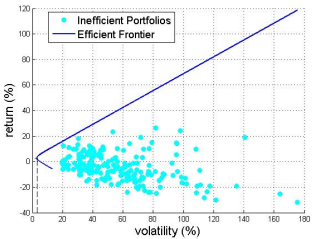
\includegraphics[scale=0.65]{img/Efficient_Frontier.png}
      \end{center}
      \end{definition}

      Note that this efficient portfolio allows us to have unlimited short positions, which may or may not be realistic. If we wanted to work only with all-long portfolios, then we would impose the nonlinear restrictions 
      \[0 \leq w_k \leq 1 \text{ for } k = 1, \ldots, K\]
      which would need to be solved numerically, possibly using nonlinear models. 

    \subsubsection{Efficient Frontier with Risk-Free Asset}

      If we include a risk-free asset such as cash $C$ with risk-free return $R_f$ to the portfolio $\{P_1, \ldots, P_K\}$, then we slightly modify our equations. By definition, the risk-free asset has volatility $\sigma_0 = 0$ and its weight must be equal to $w_f = 1 - \sum_{i=1}^K w_k$, so we still want to minimize 
      \[\sigma^2 = \frac{1}{2} \mathbf{w}^T \boldsymbol{\Sigma} \mathbf{w}\]
      subject to constraint equations 
      \[R_f \bigg( 1 - \sum_{k=1}^K w_k \bigg) + \sum_{k=0}^K w_k R_k = R\]
      When we allow our portfolio to include the risk-free security, the efficient frontier becomes a straight line that is tangential to the risky efficient frontier and with a $y$-intercept equal to the risk-free rate. 
      \begin{center}
          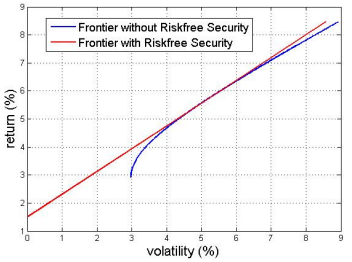
\includegraphics[scale=0.65]{img/Frontier_with_Risk_Free_Sec.png}
      \end{center}
      We can include other linear portfolio constraints, such as no-borrowing, no-short sales, or certain sector constraints. While analytic solutions are generally no longer available, the resulting problems are easy to solve numerically. 

  \subsection{Capital Asset Pricing Model}

    Let us have some stock $P$ with random variable of return $R_p = R_{P, [i, j]}$ and the market $M$ with random variable of return $R_m = R_{M, [i, j]}$, both within period $[i, j]$. There may be some sort of risk-free return $r_f$ available (e.g. U.S. treasury bonds), so we can observe the returns of these two assets past the risk-free return by considering the joint distribution 

    \begin{equation}
      (R_p - r_f) \times (R_m - r_f)
    \end{equation}

    This may or may not be correlated, but the capital asset pricing model shows that there exists a linear relationship between the expected values of these two distributions. The central insight of the CAPM is that in equilibrium the riskiness of an asset is not measured by the standard deviation of its return but by its beta. 

    \begin{theorem}[CAPM]
      Now let $\overline{R}_m = \mathbb{E}[R_m]$ denote the expected return of the market, and $\overline{R} = \mathbb{E}[R]$ denote the expected return of a security or portfolio. Then, the \textbf{capital asset pricing model (CAPM)} asserts that there exists a linear relationship 
      \begin{equation}
        \overline{R} = r_f + \beta (\overline{R}_m - r_f)
      \end{equation}
      where $r_f$ is the risk-free rate. 
    \end{theorem}
    \begin{proof}
      Let us consider a portfolio of weights $\alpha$ and $1 - \alpha$ on the risky security and market portfolio, respectively. Let $R_\alpha$ denote the random return of this portfolio as a function of $\alpha$. We then have 
      \begin{align*}
          \mathbb{E}[R_\alpha] & = \alpha \overline{R} + (1 - \alpha) \overline{R}_m \\
          \mathrm{Var}(R_\alpha) & = \alpha^2 \mathrm{Var}(R) + (1 - \alpha)^2 \mathrm{Var}(R_m) + 2 \alpha (1 - \alpha) \mathrm{Cov}(R, R_m)
      \end{align*}
      Note that as $\alpha$ varies, the mean and standard deviation $(\mathbb{E}[R_\alpha], \mathrm{Var}(R_\alpha))$ trace out a curve in $\mathbb{R}^2$ that cannot cross the efficient frontier, as shown in the dotted line. 
      \begin{center}
          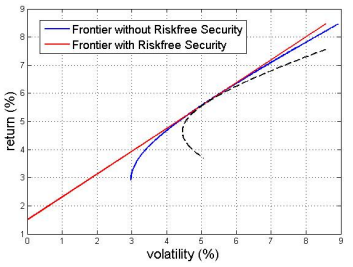
\includegraphics[scale=0.5]{img/CAPM.png}
      \end{center}
      At $\alpha = 0$, the slope of this curve must equal the slope of the capital market line. The slope of the $\alpha$-curve (where $\sigma(R_\alpha) = \sqrt{\Var(R_\alpha)}$) is 
      \begin{align*}
          \frac{d \mathbb{E}[R_{\alpha}]}{d \sigma(R_\alpha)} \bigg|_{\alpha = 0} & = \frac{d\mathbb{E}[R_\alpha]}{d \alpha} \bigg/ \frac{d \sigma(R_\alpha)}{d \alpha} \bigg|_{\alpha = 0} \\
          & = \frac{\sigma(R_\alpha) (\overline{R} - \overline{R}_m)}{\alpha \sigma(R) - (1 - \alpha) \Var (R_m) + (1 - 2 \alpha) \mathrm{Cov}(R, R_m)} \bigg|_{\alpha = 0} \\
          & = \frac{\sigma(R_m) (\overline{R} - \overline{R}_m)}{-\Var(R_m) + \mathrm{Cov}(R, R_m)}
      \end{align*}
      The slope of the capital market line is $(\overline{R}_m - r_f) / \sigma(R_m)$, and equating the two 
      \begin{equation}
        \frac{\sigma(R_m) (\overline{R} - \overline{R}_m)}{-\Var(R_m) + \mathrm{Cov}(R, R_m)} = \frac{\overline{R}_m - r_f}{\sigma(R_m)}
      \end{equation}
      gives the result. 
    \end{proof}

\section{Forward Contracts}

  

\section{Forward Contracts} 

    People trade stocks and commodities, but derivatives give more flexibility. To see why, consider the case below. 

    \begin{example}[Apples and Pies]
      Suppose you have an apple orchard and you make pies. You can sell apples and pies at a fixed price, but you can also sell them at a future price. For example, you can sell apples at a future price of \$1 per apple. 
    \end{example}

    \begin{definition}[Derivatives]
      A \textbf{derivative} is a financial instrument whose value depends on (is \textit{derived} from) the value of some other, more basic, underlying variable. Essentially, given some stochastic process $X_t$ describing some variable, the derivative is some function 
      \begin{equation}
        Y_t = g(X_t)
      \end{equation}
      The reason that we say an underlying \textit{variable} is that it includes real assets (e.g. property), financial assets (e.g. stocks), indices (stock, inflation, or housing price index), or an event (e.g. weather, or the amount of rainfall in a given season to hedge against a bad winter). Therefore, these variables can be anything, like the number of people attending a fair, which may be an indicator of the profit of the fair or some catastrophic event, and we can derive value out of that event. Therefore, the variable does not necessarily have to be an asset. 
    \end{definition}

    \begin{example}[Stock Derivative]
      For example, a stock option is derived from the value of the stock, which itself is derived from the value of the underlying company. We will see more specific examples of this later. 
    \end{example}

    \begin{example}[Weather Derivatives]
      A weather derivative can have payout of $g(S_T)$, where 
      \begin{equation}
        g(S_T) = \mathbbm{1} \{S_T > 50\} = \begin{cases} \$1 & \text{ if } S_T > 50 \\ 0 & \text{ if else} \end{cases}
      \end{equation}
      where $S_T$ is the total snowfall in inches during the year up to $T = 1$. Note that both $S_T$ and $g(S_T)$ are random variables whose value is unknown until $T = 1$.
    \end{example}

    \begin{definition}[Payoff Graph, Profit-Loss Diagram]
      To see the dependency between the underlying and the derivative, it helps to plot $g$, known as the \textbf{payoff graph}. The $x$-axis tells you the value of the underlying asset, and the $y$-axis tells you the payoff that a certain buyer or seller will make given the price of the underlying asset. 
      A \textbf{profit-loss diagram} is the same thing but it accounts for the premium paid on a contract. This is important for options since the buyer pays a premium to enter the contract, but doesn't make a difference for forward or future contracts. 
    \end{definition}

    Now we will see the most common type of derivative: the forward contract. 

    \begin{definition}[Forward Contracts]
      \textbf{Forward contracts} are simply contracts between two parties to buy or sell an asset at a future date for a price agreed upon today. 
      \begin{enumerate}
        \item $T$ is the time until delivery, usually in years. This is fixed per contract.
        \item $K$ is the delivery price. This is also fixed per contract. 
        \item $S_t$ is the spot price of the asset at time $t \in [0, T]$.
        \item $V_K (t, T)$ is the value of the contract at current time $t \leq T$ of being long a forward contract with delivery price $K$ and maturity $T$. This will vary over time. 
        \item $P(t, T)$ is the price of the forward contract at time $t$ with maturity $T$. This is the price that you pay to enter the contract.
      \end{enumerate}
    \end{definition}

    \begin{example}[Red Sox]
      If I buy the Boston Red Sox regular season wins at 90, in size one dollar per won, I have a long forward position with delivery price of 90. If the Red Sox wins 100 games I make \$10, and if they have 81 wins I lose \$9. The payout is $S_T - K$ where $S_T$ is the number of wins. 
    \end{example}

  \subsection{Primary Markets and Types of Forwards}

    \begin{example}
      We have a forward contract that agrees to buy/sell an asset for $K = \$100$ in $T=3$ months. Then, the buyer and seller have the following payoff graphs. 
      \begin{figure}[H]
        \centering 
        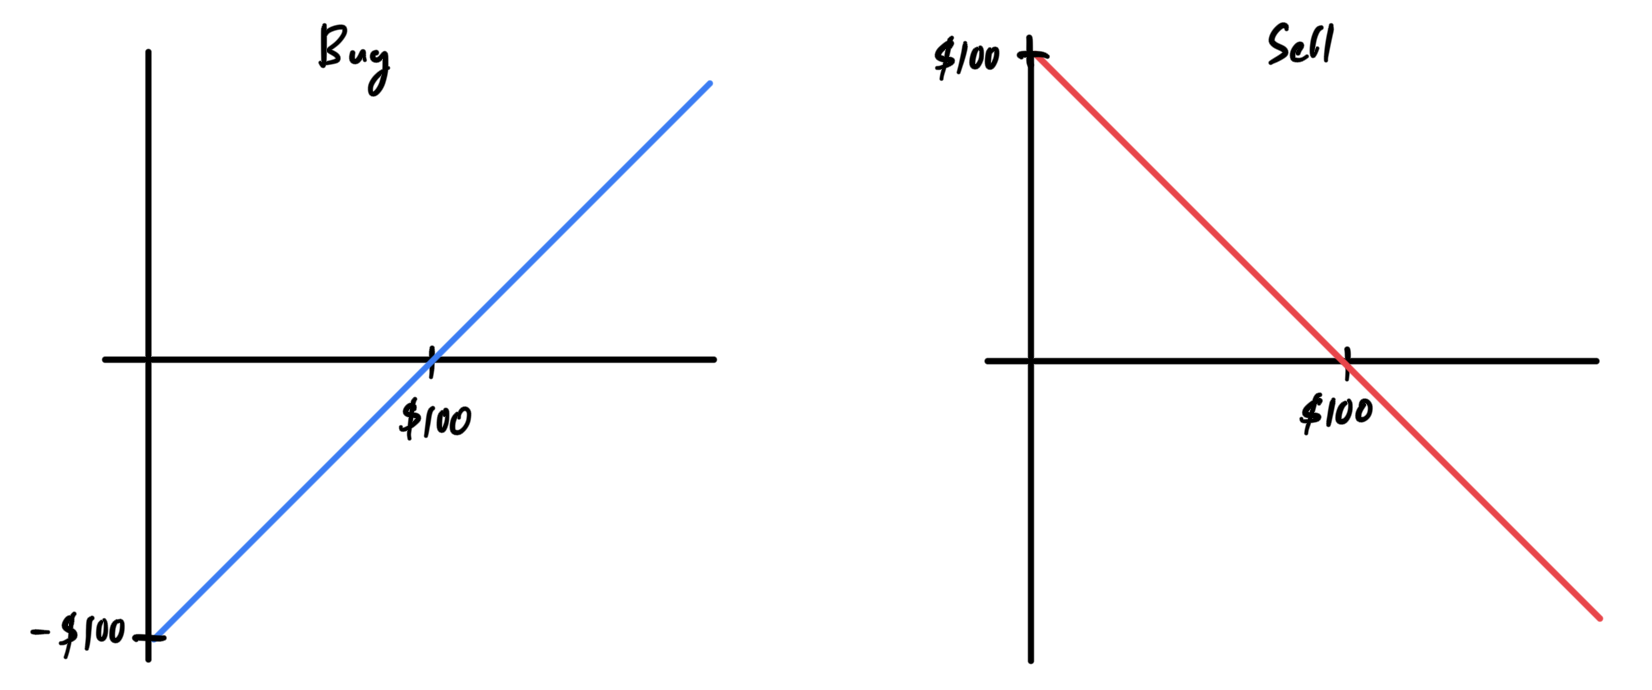
\includegraphics[scale=0.4]{img/forward_example.png}
        \caption{} 
        \label{fig:foward_example}
      \end{figure}
    \end{example}

    We can see from the following that this is a zero-sum game. Therefore, \textit{no wealth} is created or destroyed in a forward contract, it is only transferred. Since there was no cost to enter the contract, the profit is really a linear relationship between the price of the underlying asset. This is unlike options, where there is a cost to enter since the buyer or seller has the \textit{right}, but not the obligation to buy/sell the asset. This right puts an extra premium on the option that you must pay for. 

    \begin{definition}[Settlement]
      If a contract is \textbf{physically settled}, it means that the buyer actually pays $K$ and receives the asset at time $T$. However, some forwards are \textbf{cash settled}, meaning one simply receives (pays if negative) the amount $S_T - K$ at time $T$. The profit/loss is the same, but there are some key differences. 
      \begin{enumerate}
        \item A cash settled forward has no further exposure to the asset price since you're just receiving the difference in cash. However, a physically settled contract implies that the buyer now owns the asset at $T$, which continues to have exposure to asset price movements. 
      \end{enumerate}
    \end{definition}

  \subsection{Forward Contract Valuation}

    Now let's talk about how you would value a forward. 

    \begin{definition}[Value at Maturity, Payout]
      Since the party that longs the forward contract must pay $K$ at $T$ to buy an asset which is worth $S_T$, the value of the contract at $T$ is 
      \begin{equation}
        V_K (T, T) = S_T - K
      \end{equation}
      This is referred to as the \textbf{value at maturity} or the \textbf{payout} of the contract.
    \end{definition}

    \begin{definition}[Forward Price]
      The \textbf{forward price} $F(t, T)$ at the current time $t \leq T$ is the delivery price $K$ such that 
      \begin{equation}
        V_K (t, T) = 0 \implies V_{F(t, T)} (t, T) = 0 
      \end{equation}
      That is, it is the price that makes the contract have zero value at the current time. By definition, it must be the case that $F(T, T) = S_T$ since to buy an asset at $T$ for the price $F(T, T)$ is the same as buying the asset at the spot price $S_T$. 
    \end{definition}

    Since the forward price tells you what the value of the underlying asset $K$ should be at time $T$ for the contract to have no value, it is a good indicator of the actual value of the contract. When the forward is created, it has no intrinsic value, but as time goes on, the value of the contract changes as the spot price changes.

    \begin{example}
      Suppose that a stock which pays no dividends always has price $100$ and interest rates are always $0$. Then 
      \begin{enumerate}
        \item $F(t, T) = 100$ since if you had the right to buy the stock at $100$ at any time $T$, then this would be the same as buying the stock at the spot market, but it is always $100$ in the spot market. So the value of this contract must be $0$ for all $T$. 
        \item $V_K (t, T) = 100 - K$ since if you have the right to buy the stock at $K$ in time $T$, the spot price will always be worth $100$ so you're really gaining $100 - K$. Therefore the value of this contract must be $100 - K$ for all $T$. 
      \end{enumerate}
    \end{example}

  \subsection{Forward Prices}

    \begin{theorem}[Forward Price of No Income Asset]
      For an asset paying no income (e.g. a stock with no dividends), the forward price is 
      \begin{equation}
        F(t, T) = S_t e^{r (T - t)} \implies F(0, T) = S_0 e^{r T}
      \end{equation} 
    \end{theorem}
    \begin{proof}
      \textbf{Replication}. At current time $t$, let's take two portfolios. 
      \begin{enumerate}
        \item A: Consists of one unit of the underlying stock. 
        \item B: One long forward contract with delivery price $K$, plus $K e^{-r(T - t)}$ of cash. 
      \end{enumerate}
      At time $T$, B can invest the cash at the risk free rate $r$ and get $K$ cash. Then, it executes the forward contract at $K$ to get one stock. Therefore, at time $T$, both portfolios are worth $S_T$ and the values of both portfolios at time $t$ must also be the same. This is called the \textit{replication proof}. 
      \begin{equation}
        S_t = V_K (t, T) + K e^{-r (T - t)} \implies V_K (t, T)= S_t - K e^{-r (T - t)}
      \end{equation}
      We want to find the value of $K$ such that the value of the contract is $0$. Therefore, 
      \begin{equation}
        0 = S_t - K e^{-r (T - t)} \implies K = S_t e^{r (T - t)}
      \end{equation}
    \end{proof}
    \begin{proof}
      \textbf{No Arbitrage}. Another way to prove this is with the \textbf{No-arbitrage principle}. What we do is assume that the forward value is above or below our stated value, and prove that under these assumptions there is an arbitrage opportunity. 
      \begin{enumerate}
        \item Assume that $F(t, T) < S_t e^{r (T - t)}$. Then, you can buy a forward contract at delivery price $K = F(t, T)$ for free. You can also short the underlying stock at $S_t$ and invest the proceeds at the interest rate $r$. At time $T$, you can take your money, which is now worth $S_t e^{r (T - t)}$ and execute the contract by buying one share of the stock for $K = F(t, T)$. This leaves you with no stocks and money of $S_t e^{r (T - t)} - F(t, T) > 0$ by assumption, and you have an arbitrage opportunity.
        \item Assume that $F(t, T) > S_t e^{r (T - t)}$. Then, you can sell a forward contract at delivery price $K = F(t, T)$ for free. I borrow $S_t$ money at the interest rate $r$ and buy a stock. At time $T$, I sell the stock at $F(t, T)$ and also must pay back from who I borrowed at a rate of $S_t e^{r (T - t)}$. Therefore, this leaves me with a net gain of $F(t, T) - S_t e^{r (T - t)} > 0$ by assumption, and I have an arbitrage opportunity.
      \end{enumerate}
      Therefore, since I have an arbitrage opportunity, it must be the case that $F(t, T) = S_t e^{r (T - t)}$.
    \end{proof}

    Intuitively, with the no arbitrage strategy, we can see that if the forward price is too high relative to the stock price $S_t$, we buy the stock now and sell the contract (sell the stock forward at the higher price). If the forward price is too low, then we sell the stock now and buy the contract (buy the stock forward at the cheaper price). 

    \begin{corollary}[Dependence on Forward Price]
      The forward price is only dependent on the current underlying price $S_t$, the interest rate $r$, and the time to maturity $T - t$. Counterintuitively, it does not depend on the growth rate, the standard deviation, or any distributional assumptions of $S_T$. Furthermore, any two assets which pay no income and which have the same spot price $S_t$ will have the same forward price regardless of any views about their future movements. 
    \end{corollary}

  \subsection{Forward Price of Income Assets}

    However, this is unrealistic in a few things. It first does not account for dividends, the cost of storage, or the cost of carry. 

    \begin{theorem}[Forward Price of Income Asset]
      Suppose an asset pays a known amount of income (e.g. dividends, coupons, rent) during the life of the forward contract and the present value at $t$ of the income is $I$. Then, 
      \begin{equation}
        F(t, T) = (S_t - I)e^{r(T - t)}
      \end{equation}
    \end{theorem}
    \begin{proof}
      \textbf{Replication}. Let us have two portfolios. 
      \begin{enumerate}
        \item A: Consists of one unit of the underlying stock. 
        \item B: Consists of one long forward contract with delivery price $K$, plus $K e^{-r(T - t)} + I$ of cash. 
      \end{enumerate}
      Then, B will invest the cash at the risk free rate $r$ and get $K + I e^{r(T - t)}$ cash. Then it uses $K$ to buy the underlying stock, ending up with $I e^{r(T - t)}$ in cash and one unit of stock. A, by owning the stock throughout the span, also receives $I$ of cash (present value), which is equal to $I e^{r(T - t)}$ worth at time $T$. Therefore, the two portfolios are equal at time $T$ and therefore must be equal at time $t$. 
      \begin{equation}
        S_T + I e^{r(T - t)} = V_K (T, T) + K + I e^{r(T - t)} \implies S_t = V_K (t, T) + K e^{-r(T - t)} + I
      \end{equation}
      Therefore, we can solve for the forward price by setting $V_K(t, T) = 0$. 
      \begin{equation}
        S_t = K e^{-r(T - t)} + I \implies F(t, T) = K = (S_t - I) e^{r(T - t)}
      \end{equation}
    \end{proof}

    \begin{proof}
      \textbf{No Arbitrage}. We assume the two scenarios. 
      \begin{enumerate}
        \item $F(t, T) < (S_t - I) e^{r(T - t)}$. Then, we buy the forward contract for free at $K = F(t, T)$ and short the stock at $S_t$. We take the proceeds of the short and invest it at the risk free rate $r$. At time $T$, we buy back the stock at $F(t, T)$, and give back the stock to the lender, and additional pay them the dividends they would have received, which is $I e^{r(T - t)}$. Therefore, our net profit is
          \begin{equation}
            S_t e^{r(T - t)} - F(t, T) - I e^{r(T - t)} > 0
          \end{equation}
        \item $F(t, T) > (S_t - I) e^{r(T - t)}$. Then, we buy the stock at $S_t$ and short the forward contract at $K = F(t, T)$ for free. At time $T$, we get our income $I e^{r(T - t)}$, pay back the lender at $S_t e^{r(T - t)}$, and execute the contract to sell it at $F(t, T)$. Our net profit is 
          \begin{equation}
            F(t, T) + I e^{r(T - t)} - S_t e^{r(T - t)} > 0
          \end{equation}
      \end{enumerate}
      Therefore, we have an arbitrage opportunity in both cases, and therefore it must be the case that $F(t, T) = (S_t - I) e^{r(T - t)}$.
    \end{proof}

    If the stock pays some income at a componded rate, then we have the following result on the forward price. 

    \begin{theorem}
      If the stock pays a continuous dividend yield $q$ (e.g. $q = 0.02$ means that the stock pays $2\%$ of its value in dividends each year), then the forward price is 
      \begin{equation}
        F(t, T) = S_t e^{(r - q)(T - t)}
      \end{equation}
    \end{theorem}

  \subsection{Valuation of Forward Contracts}

    Recall from our example of the asset that pays no income. The replication argument gave 
    \begin{equation}
      S_t = V_K (t, T) + K e^{-r (T - t)}
    \end{equation}
    If we substitute $F(t, T) = S_t e^{r (T -t)}$ (that is, the forward price is the spot price compounded at the risk free rate), then we get
    \begin{equation}
      V_K (t, T) = (F(t, T) - K) e^{-r (T - t)} 
    \end{equation}
    which is the difference between the forward price and the delivery price, discounted back to today. 

    \begin{theorem}[Valuation of Forward Contracts]
      The value of a forward contract on an asset satisfies 
      \begin{equation}
        V_K (t, T) = \big( F(t, T) - K \big) e^{-r(T - t)}
      \end{equation}
    \end{theorem}
    \begin{proof}
      \textbf{No Arbitrage}. We assume the two scenarios.
    \end{proof}

  \subsection{Forward Interest Rates}

\section{Forward Rates and Libor}

  One might want to borrow money at a future time, say from $T_1$ to $T_2$, but they are not sure what the interest rate will be. Therefore, they can buy a forward contract that expires at $T_1$, with an underlying zero coupon bond that has maturity of $T_2$. This essentially allows them to lock in the interest rate $r_{T_1, T_2}$ for a future loan between $T_1$ and $T_2$. This is called the \textit{forward rate}. 

  \begin{definition}[Forward Rate]
    The \textbf{forward rate} at current time $t$ for period $T_1$ to $T_2$ ($t \leq T_1 \leq T_2$) is the interest rate (agreed at $t$) at which one can borrow or lend money from $T_1$ to $T_2$, i.e. the interest rate $r_{T_1, T_2}$. 

    \begin{figure}[H]
      \centering 
      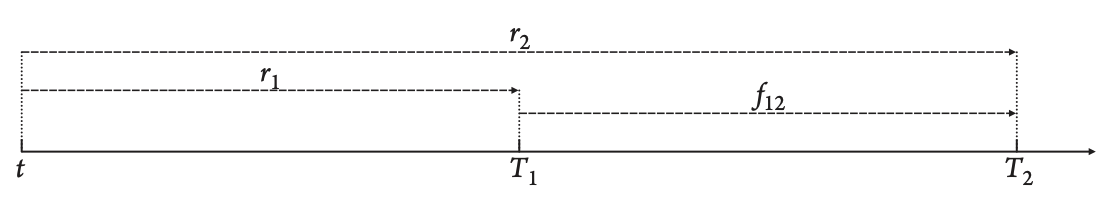
\includegraphics[scale=0.35]{img/forward_zero_rates.png}
      \caption{Letting $r_1$ be the interest rate from $t$ to $T_1$ and $r_2$ be the interest rate from $t$ to $T_2$, we can see that the forward rate $f_{12} = r_{T_1, T_2}$ is the interest rate from $T_1$ to $T_2$.}
      \label{fig:forward_zero_rates}
    \end{figure}
  \end{definition}

  A simple replication argument gives the following result about the forward rate. 

  \begin{theorem}[Forward Rate]
    At time $t$, the fair value of the forward rate $f_{12}$ is given by 
    \begin{equation}
      f_{12} = \frac{(r_2 (T_2 - t) - r_1 (T_1 - t))}{T_2 - T_1}
    \end{equation}
    if the rates of continuously compounded and 
    \begin{equation}
      f_{12} = \bigg( \frac{(1 + r_2)^{T_2 - t}}{(1 + r_1)^{T_1 - t}} \bigg)^{\frac{1}{T_2 - T_1}} - 1 
    \end{equation}
  \end{theorem}
  \begin{proof}
    By the replication argument, consider two portfolios A and B with the same money at time $t$. A first borrows money at the rate $r_1$ and then at the forward rate $f_{12}$, and B borrows at the rate of $r_2$. Then, the value of the two portfolios must be the same at time $T_2$, and so we have 
    \begin{equation}
      e_{r_1(T_1 - t)} e_{f_{12}(T_2 - T_1)} = e_{r_2(T_2 - t)} \implies f_{12} = \frac{(r_2 (T_2 - t) - r_1 (T_1 - t))}{T_2 - T_1}
    \end{equation}
    and if they are discretely compounded we have 
    \begin{equation}
      (1 + r_1)^{T_1 - t} (1 + f_{12})^{T_2 - T_1} = (1 + r_2)^{T_2 - t} \implies f_{12} = \bigg( \frac{(1 + r_2)^{T_2 - t}}{(1 + r_1)^{T_1 - t}} \bigg)^{\frac{1}{T_2 - T_1}} - 1
    \end{equation}
  \end{proof}

  \begin{theorem}[Forward Price of Zero Coupon Bonds]
    For $T_1 \leq T_2$, consider a forward contract with maturity $T_1$ on a ZCB with maturity $T_2$. That is, the underlying asset price is $S_t = Z(t, T_2)$. Then, the forward price, i.e. the price where one can (for no cost) agree to buy a forward contract on the $T_2$-ZCB with a expiry date of $T_1$, is 
    \begin{equation}
      F(t, T_1, T_2) = \frac{Z(t, T_2)}{Z(t, T_1)}
    \end{equation}
  \end{theorem}
  \begin{proof}
    Let 
    \begin{enumerate}
      \item Portfolio A be one ZCB maturing at $T_2$. 
      \item Portfolio B be one long forward with delivery price $K$, and $K$ ZCBs maturing at $T_1$. 
    \end{enumerate}
  \end{proof}

  \begin{corollary}
    Since the value of a ZCB with annually compounded rate is 
    \begin{equation}
      Z(t, T_i) = \frac{1}{(1 + r_i)^{T_i - t}} \text{ for } i = 1, 2
    \end{equation}
    we can substitute to see that the forward price of a ZCB is 
    \begin{equation}
      F(t, T_1, T_2) = \frac{Z(t, T_2)}{Z(t, T_1)} = \frac{(1 + r_1)^{T_1 - t}}{(1 + r_2)^{T_2 - t}} = \frac{1}{(1 + f_{12})^{T_2 - T_1}}
    \end{equation}
  \end{corollary}

\section{Swaps}

   

\section{Futures}

  Note that when trading futures, it is exchange traded so every trade between a buyer and a seller must go through a clearing house. Let's talk about the properties of a future contract. 

  \begin{definition}[Components of a Future Contract]
    A future contract must specify the following components. 
    \begin{enumerate}
      \item \textbf{Asset}: What is the underlying asset? 

      \item \textbf{Grade}: If the asset is a commodity, we want to specify the quality of the asset allowed at some price. Alternatively, we can talk about the \textbf{expected grade}, which allows for a range of grades depending on the actual grade of the contract.  

      \item \textbf{Contract Size}: The quantity of the asset. How much of it is being traded? The price of the contract shown is usually for one unit of the underlying commodity, so the actual value of the contract is the price times the contract size. These sizes are determined by the exchange (should be large enough for institutions to be interested in but not too big to be unaffordable). Furthermore, the mini contracts are less liquid and have a higher big ask spread. 

      \item \textbf{Delivery Location}: Where is the location? This is also standardized by the exchange, and the buyer must personally deliver the asset from these locations to wherever the asset is needed. 

      \item \textbf{Delivery Time}: The month of contract, which is the month that the commodity will be delivered and is not necessarily the same as the expiration date. 

      \item \textbf{Price Increments}: The minimum price change allowed. 

      \item \textbf{Daily Price Limits}: The maximum price change allowed in a day, and any price change beyond this limit will halt trading (called \textit{limit up} or \textit{limit down}). However, trading can still resume if it goes down. 

      \item \textbf{Position Limits}: The maximum number of contracts that a trader can hold. This is to prevent parties from cornering a market. 
    \end{enumerate}
  \end{definition}

  \begin{example}[Futures Pricing and Size Standards]
    Here is an overview of the pricing and size standards of many futures contracts set by the exchange. 

    \begin{table}[H]
      \centering
      \begin{tabular}{|l|l|l|l|}
      \hline
      \textbf{Underlying}    & \textbf{Size}      & \textbf{Increments}          & \textbf{Ex. Quote} \\ \hline
      Crude Oil (CL)        & 1000 barrels       & $1$ c ($\$10.00$)                 & $\$86.73$\\ \hline
      Crude Oil (CL) Mini   & 500 barrels        & $1$ c ($\$5.00$)                  & $\$86.73$ \\ \hline
      Natural Gas (NG)      & 10,000 mmBtu       & $\sfrac{1}{10}$ c ($\$10.00$)  & $\$2.843$ \\ \hline
      Corn (ZC)             & 5000 Bushels       & $\sfrac{1}{8}$ c ($\$12.50$)   & $400\sfrac{3}{8}$ c \\ \hline
      Wheat (ZW)            & 5000 Bushels       & $\sfrac{1}{8}$ c ($\$12.50$)   & $568\sfrac{1}{4}$ c\\ \hline
      Soybean (ZS)          & 5000 Bushels       & $\sfrac{1}{8}$ c ($\$12.50$)   & $1655\sfrac{1}{2}$ c\\ \hline
      Gold (CS)             & 100 Troy Ounces    & $10$ c ($\$10.00$)                & $\$2349.10$\\ \hline
      Silver (SI) Full      & 5000 Troy Ounces   & $\sfrac{1}{10}$ c ($\$5.00$)   & $\$27.247$ \\ \hline
      Silver (SI) Micro     & 1000 Troy Ounces   & $\sfrac{1}{10}$ c ($\$1.00$)   & \\ \hline
      Copper (NG)           & 25,000 Pounds      & $\sfrac{1}{200}$ c($\$12.50$)  & \\ \hline
      E-Mini S\&P 500       & 50                 & $0.25$ c ($\$12.50$)             & \\ \hline
      E-Mini Nasdaq 100     & 20                 & $0.25$ c ($\$5.00$)              & \\ \hline
      E-Mini Dow            & 5                  & $1$ c ($\$5.00$)                 & \\ \hline 
      E-Mini Russell 2000   & 50                 & $0.10$ c ($\$5.00$)              & \\ \hline
      Micro E-Mini S\&P 500 & 5                  & $0.25$ c ($\$1.25$)              & \\ \hline
      Micro E-Mini Nasdaq 100 & 2                & $0.25$ c ($\$0.50$)              & \\ \hline
      Micro E-Mini Dow      & 0.5                & $1$ c ($\$0.50$)                 & \\ \hline
      Micro E-Mini Russell 2000 & 5              & $0.10$ c ($\$0.50$)              & \\ \hline
      Treasury Bonds        & \$100,000          & $\frac{1}{32}$ c ($\$31.25$)   & \\ \hline
      Treasury Bonds        & \$200,000          & $\frac{1}{32}$ c ($\$62.50$)   & \\ \hline
      \end{tabular}
      \caption{Standards of Futures Contracts}
      \label{tab:futures_standards}
    \end{table}

    \begin{enumerate}
      \item \textbf{Corn} is delivered to Toledo, Ohio. 
      \item \textbf{Oil} (WTI) is delivered to Cushing, Oklahoma.
    \end{enumerate}

    \begin{enumerate}
      \item For oil, natural gas, and copper, the delivery month is the month after the expiration month and delivers on all months. 
      \item For corn, wheat, and soybean, we only deliver on the months of March, May, July, September, and December.
    \end{enumerate}
  \end{example}

  \begin{example}[Harvest and Delivery Standards]
    While most futures deliver throughout the year, for grain (corn, wheat, soybean) futures, they deliver on  the months of March, May, July, September, and December. This is because these are the months of the harvest.
  \end{example}

  It turns out that this discrepancy is important in analyzing the convergence of the future price to the spot price and determining the risk. 

\section{Options}

  \begin{definition}[Long Options]
    An option is a contract that gives the owner the right, but not the obligation, to buy or sell a specific asset (the \textbf{underlying}) at a specific price $K$ (\textbf{strike} or \textbf{exercise price}) at a specific date $T$ (\textbf{expiration date}). When you buy (long) 
    \begin{enumerate}
      \item a \textbf{call option} for $\$X$, then you have the \textit{right} to buy the asset and the seller has the \textit{obligation} to sell. 
      \begin{figure}[H]
        \centering 
        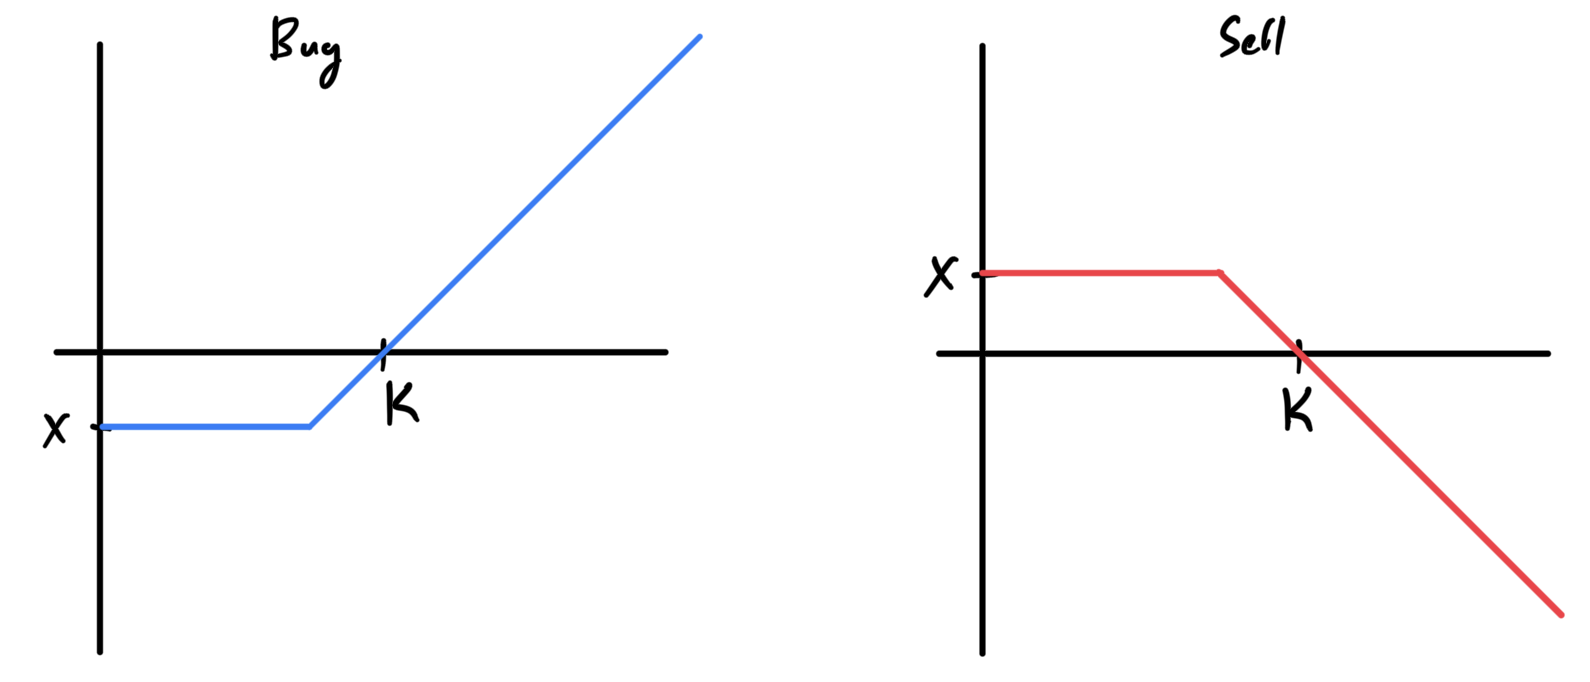
\includegraphics[scale=0.4]{img/call_options.png}
        \caption{Note that the buyer has limited loss and has unlimited gain with the long put, while the seller has limited gain and unlimited loss with the short put.} 
        \label{fig:call_options}
      \end{figure}
      \item a \textbf{put option} for $\$X$, then you have the \textit{right} to sell the asset and the seller has the \textit{obligation} to buy. 
      \begin{figure}[H]
        \centering 
        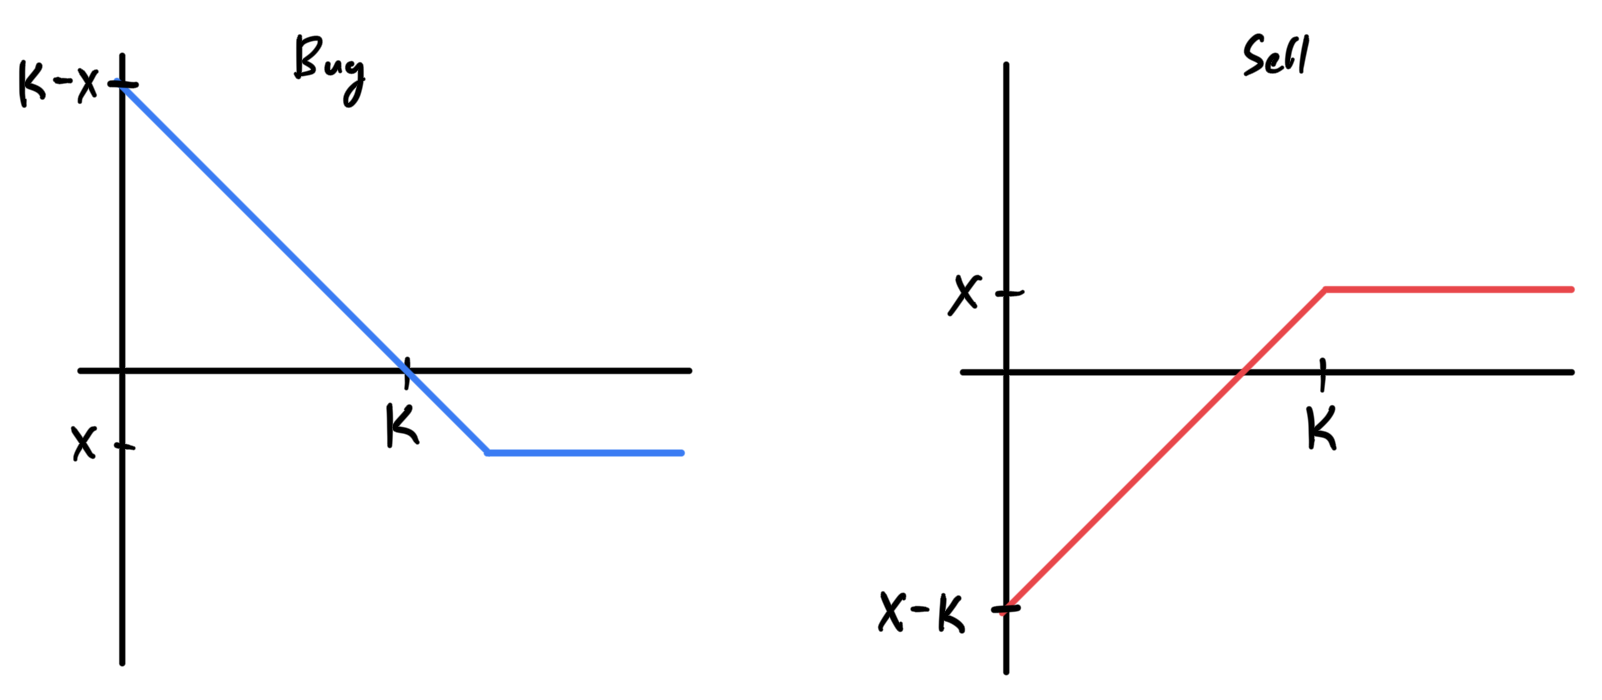
\includegraphics[scale=0.4]{img/put_options.png}
        \caption{Note that the buyer has limited loss and limited gain, and the seller also has limited loss and limited gain. } 
        \label{fig:put_options}
      \end{figure}
    \end{enumerate}
    There are three types of options. 
    \begin{enumerate}
      \item \textbf{American style} options can be exercised anytime during the life of the option. 
      \item \textbf{European style} options can only be exercised at the expiration date.
      \item \textbf{Bermuda style} options can be exercised at specific dates during the life of the option.
    \end{enumerate}
    This has nothing to do with which continent the options are trading in. It is just a name. Most exchange traded options are American style and most OTC options are European style. 
  \end{definition}

  Note that unlike forwards or futures, the premium changes hands, i.e. the buyer pays the seller to enter the contract.  

\section{Exercises}

  \begin{exercise}[Hull 1.3]
    What is the difference between entering in to a long forward contract when the forward price is $\$50$ and taking a long position in a call option with a strike price of $\$50$? 
  \end{exercise}
  \begin{solution}
    The answer is clear when we look at the payoff graph for each one.  
    \begin{enumerate}
      \item The first difference is that the forward contract renders both parties obligated to buy or sell the underlying at a future time, while the option only gives the seller the obligation to sell, if the buyer requests it.  
      \item The second is that money is paid to enter into the options contract by the buyer, while the forward contract does not. 
      \item Both profits/losses are unlimited in the forward contract, while in the options contract, the buyer has limited loss and the seller has unlimited loss. 
      \item By having the safety of a limited downside for the call options buyer, they get a slightly lower payoff $S_T - C_0$ compared to the forward contract, which is $S_T$. Therefore, the options buyer doesn't actually make a profit until the price of the underlying asset is at least $C_0 + K$. 
      \item If $S_T > K$, we would wish we were taking the forward, and if $S_T < K$, then we wish we were taking the call option.  
    \end{enumerate}
    \begin{figure}[H]
      \centering 
      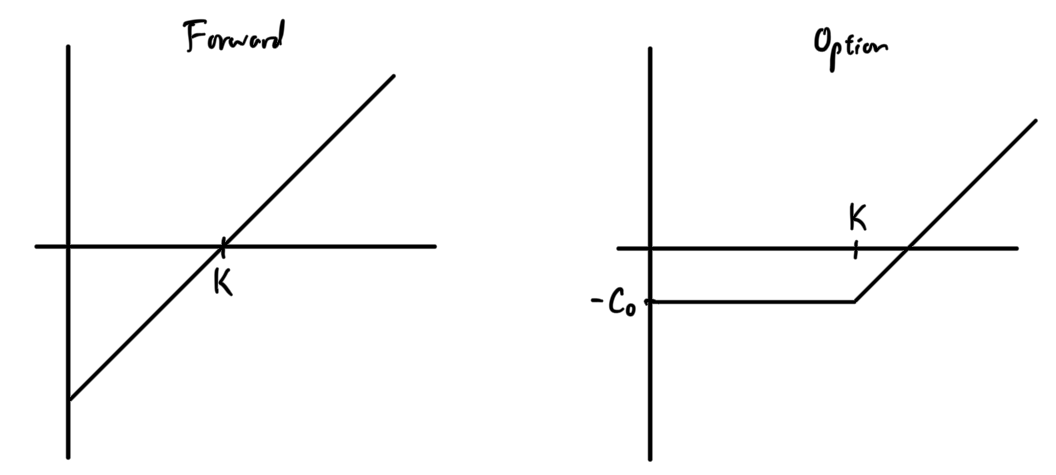
\includegraphics[scale=0.4]{img/ex1-3.png}
      \caption{The payoff graph for the forward contract and the call option from the buyers side.} 
      \label{fig:ex1-3}
    \end{figure}
  \end{solution}

  \begin{definition}[Pips]
    For the next problem, it helps to know that a \textbf{pip} is 1/100 of a cent. 
  \end{definition}

  \begin{exercise}[Hull 1.5]
    An investor enters into a short forward contract to sell $100,000$ British Pounds for US dollars at an excahnge rate of $1.5$ dollars per pound. How much does the investor gain or lose if the exchange rate at the expiration date is $1.4900$ dollars per pound? What if it is $1.5200$ dollars per pound? 
  \end{exercise}
  \begin{solution}
    Note that we must specify the currency of the profit or loss. It turns out that the payoff will always be in the currency that the investor is selling. The investor is selling the forward, so they are obligated to sell it at $1.5000$ dollars per pound. 
    \begin{enumerate}
      \item If the rate is $1.4900$, then the investor sells the pounds for $150,000$ USD and can buy a little bit more than $100,000$ pounds. In fact, they are making a profit of $100,000 \cdot 0.0100 = 1,000$ dollars.
      \item If the rate is $1.52$, then the investors sells the pounds for $150,000$ USD and can buy a little less than $100,000$ pounds, so they lose $100,000 \cdot 0.0200 = 2,000$ dollars. 
    \end{enumerate}
  \end{solution}


  \begin{exercise}[Hull 1.6]
    A trader enters into a short cotton futures contract when the futures price is 50 cents per pound. The contract is for the delivery of 50,000 pounds. At the end of the contract, the price of cotton is $48.20$ or $51.30$ per pound. What is the trader's gain or loss?
  \end{exercise}
  \begin{solution}
    The trader is selling the cotton, and the buyer is obligated to buy. Therefore, 
    \begin{enumerate}
      \item the trader makes $(50 - 48.20) \cdot 50,000 = 1.8 \cdot 50,000 = 90,000$ cents, or $\$900$ if the price is $48.20$. 
      \item the trader loses $(51.30 - 50) \cdot 50,000 = 1.3 \cdot 50,000 = 65,000$ cents, or $\$650$ if the price is $51.30$.
    \end{enumerate}
  \end{solution}

  \begin{exercise}[Hull 1.16]
    A trader writes (sells) a December put option with a strike price of $\$30$. The price of the option is $\$4$. Under what circumstances does the trader make a profit? 
  \end{exercise}
  \begin{solution}
    Even without a payoff graph, we can see that since I'm selling the option, I'm getting $\$4$. Now, I'm obligated to buy the asset (since it's a put) at $\$30$, and therefore I will profit if the price of the asset is above $\$30$. However, since I already have the cushion of $\$4$, I'm really profiting if the asset price $S_T > 26$. 
    \begin{figure}[H]
      \centering 
      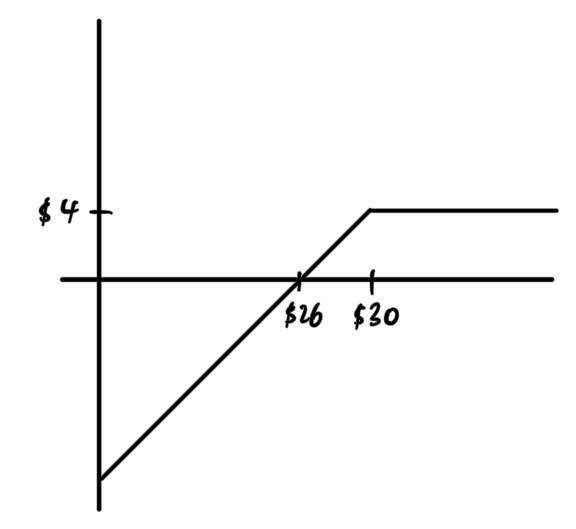
\includegraphics[scale=0.2]{img/ex1-16.png}
      \caption{The payoff graph for the put option from the sellers side.} 
      \label{fig:ex1-16}
    \end{figure}
  \end{solution}

  \begin{exercise}[Hull 1.22]
    I am in a long forward contract and a long put option at the same strike price $K$. What is the payoff of this position at expiration?
  \end{exercise}
  \begin{solution}
    You can simply draw the profit-loss diagram. 
    \begin{figure}[H]
      \centering 
      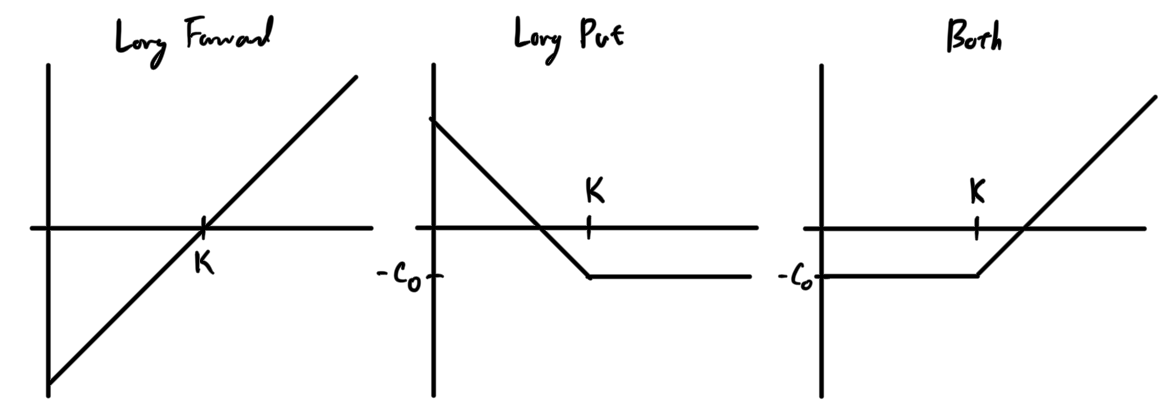
\includegraphics[scale=0.2]{img/ex1-22.png}
      \caption{The payoff graph for the long forward and long put option at the same strike price.} 
      \label{fig:ex1-22}
    \end{figure}
  \end{solution}

  \begin{exercise}[Hull 1.23]
    We have a \textbf{Index Currency Option Note (ICON)} which states the following: 
    \begin{enumerate}
      \item If the exchange rate USD.JPY $ < 169$, then the bond pays $1000$ USD.
      \item If $84.50 \leq USD.JPY \leq 169$, then the bond pays 
        \begin{equation}
          1000 - \max\bigg\{ 0, 1000 \Big( \frac{169}{S_T} - 1 \Big)\bigg\}
        \end{equation}
      \item If $USD.JPY < 84.50$, then the bond pays nothing. 
    \end{enumerate}
    Show that this ICON is a combination of a bond and two options. 
  \end{exercise}
  \begin{solution}
    This seems a bit easy since we can draw the payoff diagram as such. 
    \begin{figure}[H]
      \centering 
      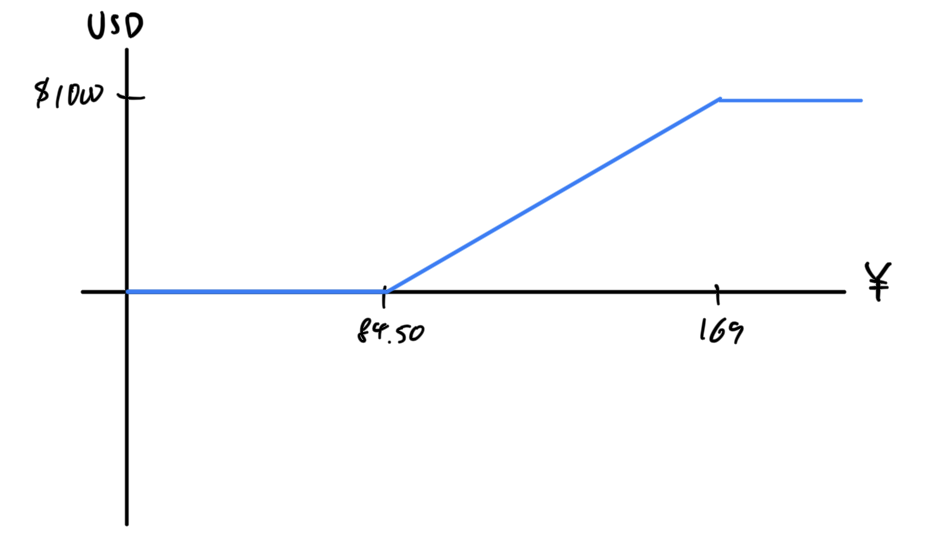
\includegraphics[scale=0.2]{img/ex1-23-1.png}
      \caption{} 
      \label{fig:ex1-23-1}
    \end{figure}
    However, the underlying asset is shown in yen and the payoff in USD, which complicates calculations. You should rather change the underlying to be USD by changing USD.JPY to JPY.USD. Then, we can do some quick sketches to find that you should have a 
    \begin{enumerate}
      \item Bond at $\$1000$. 
      \item Short call at $1/169$ for $\$1000$. 
      \item Long call at $1/84.50$ for $\$1000$.
    \end{enumerate}
    \begin{figure}[H]
      \centering 
      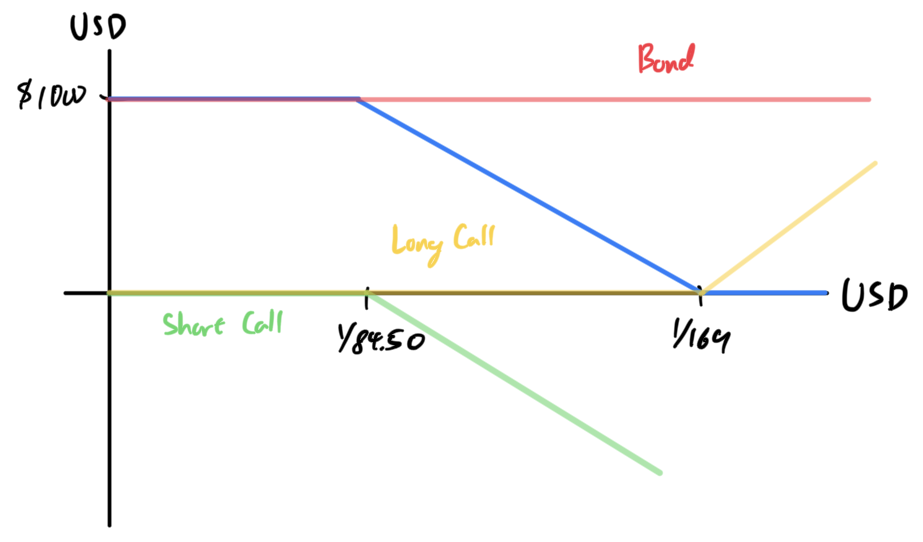
\includegraphics[scale=0.2]{img/ex1-23-2.png}
      \caption{} 
      \label{fig:ex1-23-2}
    \end{figure}
  \end{solution}

\section{Appendix}

  Futures are mostly cash settled (e.g. look at futures on SP500 index. you can't deliver fractional shares. )

  Margin calls with futures. 

  The difference between the spot and the futures price is called the basis gap/risk. They tend to converge as we approach the expiration date. 

  Order types (market, limit - default, stop), which exists for both long and short futures. 

  Regulations are done by the CFTC (Dodd-Frank Act expands CFTC oversight to OTC markets due to 2008). Accounting (does unrealized gains count as taxable income?) and taxes can be country specific. 

  Talk about derivatives in general 
  - stuff like payoff graphs 
  - definitions of derivatives 

  Forwards \& Futures 
  - how they work, with trading, delivery, quality of goods, settlement (delivery or cash settled). Does delivery actually happen? You must actually request to have it delivered to a warehouse you set up. This could have inventory/delivery fees as well.  
  - basis risk (spot price of asset $A$ is $S_A$, and the futures is $F_A$). (8)
  - hedging strategies with futures (short \& long futures) hedge ratio, with cross-hedging, and minimizing the variance of our position. (is this delta-hedging?) 
  - stock index futures (you need CAPM to evaluate this)




\end{document}
